\documentclass{article}
\usepackage[utf8]{inputenc}
\usepackage{hyperref}
\usepackage{float}
\usepackage[table,xcdraw]{xcolor}
\usepackage{color, colortbl}
\usepackage{longtable}
\usepackage{booktabs}
\usepackage{graphicx}
\usepackage{multirow}
\usepackage{tikz}
\usepackage{rotating}
\usepackage{caption}
\usepackage{authblk}
\graphicspath{{Figures/}}
\usepackage{rotating}
\usepackage{geometry}
\usepackage{array}
\usepackage{lscape}
\usepackage{longtable}
\usepackage{hhline}
\usepackage{lmodern}
\usepackage[
backend = biber,
natbib,
style = apa,
citestyle = authoryear,
maxcitenames = 2, 
maxbibnames = 99, 
uniquename=false,
uniquelist=false
%sorting = none % sort by name year title
]{biblatex}
\addbibresource{Ref_invertebrate_DB.bib}

%%%%%%%%%%%%%%%%%%%%%%%%%%%%%%%%%%%%%%%%%%%%%%%%%%%%%%%%%%%%%%%%%%%%%%%%%%%%%%%%%%%%%%%%%%
% From freshwater biology:
% List all sources in the reference list alphabetically by name. In text citations should follow the author-date method. This means that the author's last name and the year of publication for the source should appear in the text, for example, (Jones, 1998), and a complete reference should appear in the reference list at the end of the paper.

% References are styled according to the sixth edition of the Publication Manual of the American Psychological Association. A sample of the most common entries in reference lists appears below. Please note that for journal articles, issue numbers are not included unless each issue in the volume begins with page one.

% Article: 
% One author: Fawcett, T. (2006). An introduction to ROC analysis. Pattern Recognition Letters, 27(8), 861–874. DOI: 10.1016/j.patrec.2005.10.010.

% 2 to 7 authors: Daley, C. E., & Nagle, R. J. (1996). Relevance of WISC-III Indicators for assessment of learning disabilities. Journal of Psychoeducational Assessment, 14 (4), 320–333.

% More than 7 authors: Rutter, M., Caspi, A., Fergusson, D., Horwood, L. J., Goodman, R., Maughan, B., … Carroll, J. (2004). Sex differences in developmental reading disability: New findings from 4 epidemiological studies. Journal of the American Medical Association, 291(16), 2007–2012. DOI: 10.1001/jama.291.16.2007

% In press or forthcoming: van Bergen, E., de Jong, P. F., Maassen, B., Krikhaar, E., Plakas, A., & van der Leij, A. (in press). IQ of four-year-olds who go on to develop dyslexia. Journal of Learning Disabilities. DOI: 10.1177/0022219413479673
%%%%%%%%%%%%%%%%%%%%%%%%%%%%%%%%%%%%%%%%%%%%%%%%%%%%%%%%%%%%%%%%%%%%%%%%%%%%%%%%%%%%%%%%%%


\usepackage{subfiles} % Best loaded last in the preamble

% functions and definitions
\definecolor{Gray}{gray}{0.9}

% horizontal space between two columns
\setlength{\tabcolsep}{2mm}

\newcommand{\specialcell}[2][c]{%
  \begin{tabular}[#1]{@{}c@{}}#2\end{tabular}}

\renewcommand*{\thefootnote}{\alph{footnote}}


%%%%%%%%%%%%%%%%%%%%%%%%%%%%%%%%%%%%%%%%%%%%%%%%%%%%%%%%%%%%%%%%%%%%%%%%%%%%%%%%%%
%%%%%%%%%%%%%%%%%%%%%%%%%%%%%%%%%%%%%%%%%%%%%%%%%%%%%%%%%%%%%%%%%%%%%%%%%%%%%%%%%%
\title{Tackling discrepancies in freshwater invertebrate trait databases: Harmonising across continents and aggregating taxonomic resolution}
\author[1]{Stefan Kunz}
\author[2]{Ben J. Kefford}
\author[3]{Leon Metzeling}
\author[4]{Astrid Schmidt-Kloiber}
\author[4]{Wolfram Graf}
\author[5]{Philippe Usseglio-Polatera}
\author[6]{Christoph D. Matthaei}
\author[7]{Charles P. Hawkins}
\author[8]{N. LeRoy Poff}
\author[9]{Laura Twardochleb}
\author[1]{Ralf B. Schäfer}
\affil[1]{Institute for Environmental Sciences, University of Koblenz-Landau, Landau, Germany}
\affil[2]{Centre for Applied Water Science, Institute for Applied Ecology, University of Canberra, Canberra, Australia}
\affil[3]{Environment Protection Authority Victoria, Applied Sciences Division, Macleod, Australia}
\affil[4]{Institute of Hydrobiology and Aquatic Ecosystem Management, University of Natural Resources and Life Sciences Vienna (BOKU), Vienna, Austria}
\affil[5]{University of Lorraine, CNRS, LIEC, Metz, France}
\affil[6]{Department of Zoology, University of Otago, Dunedin, New Zealand}
\affil[7]{Department of Watershed Sciences and the Ecology Center, Utah State University, Logan, USA}
\affil[8]{Department of Biology, Colorado State University, Fort Collins, USA}
\affil[9]{Department of Fisheries and Wildlife, Michigan State University, East Lansing, USA}
\date{}

\begin{document}
\maketitle

\newpage

\section*{Abstract}

% FROM FRESHWATER BIOLOGY Website:
% All papers should include a summary, in short numbered paragraphs, limited to about 3% of the length of the text, and in any case to not more than 500 words. This should provide a concise statement of the scope of the work and its principal findings and be fully intelligible without reference to the main text. It is helpful to structure your abstract as follows: point 1 = background to and reason for the study and the aims; point 2 = brief description of methods used; point 3 = main project results (address the aims); point 4 = conclusions of your study; point 5 = the contribution that your results make to the field / why your study is useful to an international audience. Referring to abstracts in recently published issues may help with structuring an abstract.


% Alternative start: Invertebrate traits are increasingly used in ecological studies because they provide a mechanistic understanding of species-environment relationships and are suitable for large scale analysis due to their consistent response to environmental gradients.

1. Use of invertebrate traits rather than species composition may facilitate large-scale comparisons of community structure and responses to disturbance in freshwater ecology because the same traits can potentially occur everywhere.  In recent years, comprehensive invertebrate trait databases have been established at different scales (e.g. regions, continents). The wide availability of invertebrate trait data supports trait-based studies, especially at large scales. However, a number of data-related issues complicate the use of invertebrate traits for ecological studies. For example, standardised definitions for for freshwater invertebrate traits are lacking, which impedes comparisons across regions. Moreover, it is uncertain how harmonising varying trait definitions among databases might influence identification of trait-environment relationships. In addition, taxonomic resolution between observational taxonomic data and trait data can differ, making aggregation of traits necessary. At present, it is unknown how different trait aggregation approaches compare with expert-assigned trait affinities. In this study we aimed to identify discrepancies in trait definitions across freshwater invertebrate databases and to compare trait aggregation methods to identify how taxonomic hierarchy structure and trait variability influence results from different aggregation approaches.

2. We describe discrepancies in the definitions of traits used to create freshwater invertebrate trait databases in Europe, North America, New Zealand, and Australia. Based on our comparisons of these trait databases, we established four novel trait datasets by harmonising trait definitions of commonly used traits. Next, we used two of these datasets to compare aggregated traits obtained by different aggregation methods with traits assigned by experts, both at the family level. The trait aggregation methods we compared used either the mean or the median and different weightings. We further explored the effects of harmonisation and trait aggregation by re-analysing data from a case study.

3. We found that among trait databases, trait definitions often differed because varying numbers of traits were used to describe groups of related traits (e.g., respiration traits) and the focus of descriptions for groups of related traits also varied (e.g., for feeding mode some databases focused on the food source, whereas others focused on mouthpart morphology). The coding to describe traits (binary, fuzzy) also varied among databases. Our comparison of different aggregation methods showed that family-level aggregated and expert-assigned traits were similar, especially from approaches using the median, and that trait coding method, uneven taxonomic hierarchical structure, and high trait variability can influence aggregated trait affinities. We further showed that harmonised and aggregated data performed similarly to observational data in identifying trait–environment relationships.

4. By outlining discrepancies in trait definitions we hope to motivate the development of standardised terminology for invertebrate traits. Our results also illustrate the usefulness of harmonised datasets for ecological study and provide guidance for the circumstances under which the choice of trait aggregation method is important.


\newpage

\section*{Introduction}

Explaining and predicting how communities are shaped by environmental factors is a primary main goal of ecology. Species traits are measurable properties of an organism (\cite{mcgill_rebuilding_2006}), and comparing communities based on the traits possessed by species may facilitate testing of a range of ecological hypotheses (\cite{heino_jani_macroecological_2013}). Traits are assumed to be adaptations (e.g., physiological, behavioural) of organisms to their environment and to indicate direct or indirect linkages between the biological response of an organism or a population and its environment (\cite{southwood_habitat_1977, verberk_delivering_2013}).
In addition to providing local-scale mechanistic-based expressions of species-environment relationships, trait-based approaches might be suitable for large-scale analyses because trait responses are less constrained by biogeographic boundaries and taxon distributional areas than taxonomic responses (\cite{baird_toward_2011, bonada_taxonomic_2007}). 

Invertebrate traits have been increasingly used in freshwater ecology, e.g. by relating macroinvertebrate trait composition to environmental factors (\cite{bhowmik_large_2015, poff_developing_2010, szocs_effects_2014}). In the last decades, freshwater ecologists have compiled comprehensive invertebrate trait databases, which typically include data for a single region or continent (\cite{kefford_integrated_2020, Philips_and_Smith_NZ_DB_2018, schmidt-kloiber_www.freshwaterecology.info_2015, tomanova_trophic_2006, ussegliopolatera_biological_2000, vieira_database_nodate}). The availability of invertebrate trait data from different continents enables comparisons of regional trait variation and allows for testing the consistency of trait structure–environmental factor relationships across both small and large spatial extents. To date, such analyses have been carried out mostly within continents, using information from one or two trait databases. For example, \citet{bonada_taxonomic_2007} compared trait composition for Mediterranean and temperate regions in Europe based on traits from \citet{ussegliopolatera_biological_2000} (typically referred to as the Tachet database), \citet{poff_developing_2010} characterized trait composition across sites in the Western USA based on traits from \citet{poff_functional_2006}, and \citet{botwe_effects_2018} used trait definitions from \citet{poff_functional_2006} and \citet{schafer_trait_2011} to test for effects of salinity on invertebrate traits across different sites in South Australia. Analyses that synthesize invertebrate trait information from more than two different continents are rare, but see \citet{brown_functional_2018} and \citet{statzner_reproductive_1997}. 

The heterogeneity of information in freshwater invertebrate trait databases, besides the diversity of taxa across regions, is likely a major reason for the lack of studies across continents. There are several challenges presented by using invertebrate trait data from multiple established databases in ecological studies. One such challenge is inconsistency in terminology. In this study, we follow the terminology proposed by \citet{schmera_proposed_2015}, where a grouping feature is defined as a general property (e.g. feeding mode) that comprises a "group of related traits (e.g., predator, shredder, etc.) that vary among species or among individuals within a species". Thus, we use the term grouping feature in place of the term trait, and the term trait instead of trait state, modality or trait category. 

Another challenge to using data from multiple continents is that invertebrate trait databases include different grouping features and related traits. To harmonize grouping features from different regions, or to structure them in such a way as to facilitate cross-database comparison, commonly accepted and unambiguous trait definitions are required (\cite{schneider_towards_2019}). Ideally, the same traits and grouping features would be reported across databases or standardised terminology would exist to easily harmonise them; however, there is a lack of standardised terminology of trait definitions and poor metadata quality in many trait databases, making grouping-feature harmonisation difficult (\cite{baird_toward_2011, kissling_towards_2018}). To our knowledge, only \citet{brown_functional_2018} harmonised grouping features from more than two geographically distant invertebrate trait databases, for a limited set of grouping features (8) and taxa (112), in a study on the influence of decreasing glacier cover on functional diversity and invertebrate assemblages.

A third challenge to comparing across invertebrate trait databases is inconsistent coding of trait data (\cite{culp_incorporating_2011}), or assigning affinities (aka affinity scores). Traits of individual freshwater invertebrates can be difficult to quantify because, unlike plant traits, they are often difficult to measure directly. For example, to describe feeding habits requires that we understand mouthpart morphology, feeding behaviour, and specific food sources (\cite{moog_comprehensive_nodate}). Some traits can be described as binary or categorical, which ignores uncertainty in how traits are expressed in any particular organism (e.g., adult terrestrial stage, presence of gills). Other traits are better suited to being described as continuous (e.g., tolerance of pollution, body size). One approach for dealing with uncertainty is the use of fuzzy coding, where traits are assigned probabilistic values. Fuzzy codes, which are usually converted to proportions, are used to account for plasticity in traits, variability in traits within taxonomic groups above the species level, and incomplete knowledge. A challenge is presented by the use of different types of coding for trait affinities in different databases. For example, in the study from \citet{brown_functional_2018} the authors needed to reclassify trait affinities because the individual databases employed different coding approaches (i.e., European and New Zealand databases used fuzzy coding, North American database used binary coding). 

Finally, discrepancies in the taxonomic resolutions (e.g., species, genus, or family) when comparing among trait databases, or when linking observational taxonomic data to trait databases, presents another challenge. When observations or data in one trait database are at a more precise taxonomic level than other data (e.g. observations at species-level and trait data at genus-level) trait information of the less precise taxonomic level is often assigned (e.g. \cite{szocs_effects_2014, vos_taxonomic_2017}). Conversely, if trait information is only available at more precise taxonomic levels than observed taxa, traits are aggregated to a less precise taxonomic level (e.g. \cite{aspin_extreme_2019, piliere_a._f._h._importance_2016, poff_functional_2006, szocs_effects_2014}). To date, studies have used different methods of trait aggregation, e.g. the mean (\cite{magliozzi_functional_2019}), median (\cite{szocs_effects_2014}) or mode (\cite{piliere_a._f._h._importance_2016}), but studies on how and to what extent different trait aggregation methods influence trait-based analyses are missing. 
%However, related knowledge would inform future studies regarding the choice of the aggregation method.

These challenges when working with or synthesizing trait data motivated us to assess the characteristics and comparability of freshwater invertebrate trait data contained in disparate databases. We aimed to explore methods of improving the comparability of trait data across databases, despite differences in trait definitions and the taxonomic level of data in three ways: (1) by investigating and describing discrepancies in trait definitions between trait databases from Europe, North America, Australia, and New Zealand; (2) by harmonising trait definitions across databases to provide consistent trait grouping features for comparison across geographic locations; and (3) by comparing the influence of different trait aggregation methods and grouping-feature harmonisation on the identification of trait–environment relationships.

% Other alternative from Brooke: These challenges when working with or synthesizing trait data motivated us to assess the characteristics and comparability of freshwater invertebrate trait data contained in disparate databases. We aimed to explore methods of improving the comparability of trait data across databases, despite differences in trait grouping-feature definitions, affinity score coding, and taxonomic level of data, through two study objectives: (1) to investigate the plausibility of comparing across databases from different geographic regions by providing harmonised datasets from Europe, North America, Australia, and New Zealand; and (2) to compare the influence of different trait aggregation methods on the characterisation of trait–environment relationships.


\newpage
%%%%%%%%%%%%%%%%%%%%%%%%%%%%%%%%%%%%%%%%%%%%%%%%%%%%%%%%%%%%%%%%%%%%%%%%%%%%%%%%%%%%%%%%%%%%%%%%%%%%%

\section*{Methods}

%Version from Brooke: As a basis for evaluating the comparability of freshwater invertebrate databases, we developed four novel invertebrate trait datasets by harmonising seven grouping features from existing trait databases. We then evaluated the influence of different...

To address our study objectives, we took a multi-prong approach to describing, combining, and assessing multiple sources of freshwater invertebrate data that differed in grouping-feature definitions and taxonomic resolution. Identified trait definitions discrepancies served as a starting point to develop four novel invertebrate trait datasets by harmonising seven grouping features from existing trait databases. The harmonised trait datasets were used to evaluate the influence of different trait aggregation approaches on the identification of trait–environment relationships, our third study objective, in two ways by (1) comparing family-level aggregated trait affinities with family-level trait affinities assigned by experts for two of the established trait datasets where such data were available and (2) comparing the influence of taxonomic hierarchy and trait variability on the outcomes of the different trait aggregation approaches for simulated data. Finally, to further investigate how harmonising and aggregating trait data can modify the outcomes of trait–environment relationship characterisation, we used data from one of the newly established datasets with harmonised and aggregated traits to repeat an analysis of salinisation effects on biological traits (\cite{szocs_effects_2014}) and compared our results with those of the original study.

\subsection*{Selection of traits and harmonisation of trait databases}

To explore the characteristics and comparability of freshwater invertebrate trait data with differing grouping-feature definitions and taxonomic resolution, we obtained invertebrate trait data from six trait databases for four regions: Europe, North America, Australia, and New Zealand. For Europe we obtained trait information from the freshwaterecology.info database (\cite{schmidt-kloiber_www.freshwaterecology.info_2015}), which contains taxa at the species level, and the Tachet database (\cite{ussegliopolatera_biological_2000}), which contains taxa at species, genus, and family levels. For North America we primarily obtained trait information from \citet{twardochleb_freshwater_nodate} (hereafter referred to as the CONUS database) and where taxa were missing from that database, we obtained data from \citet{vieira_database_nodate} (hereafter referred to as the Vieira database). Both databases contain taxa at species, genus and family levels. Data on body form for European and North American taxa were based on expert knowledge (\cite{polatera_personal_information_2020}). For Australia and New Zealand, we used trait databases from \citet{kefford_integrated_2020} (hereafter referred to as the Australian database) and \citet{Philips_and_Smith_NZ_DB_2018} (hereafter referred to as the New Zealand database) respectively. These databases contain taxa at species, genus, family, and less precise taxonomic levels.

We established four datasets, one for each of the four geographic regions, by harmonising the traits of seven grouping features from the trait databases. We selected traits that were available in all databases, are commonly applied in trait-based ecological studies, and describe different parts of the biology of a species: life history (Voltinism), morphology (Respiration, Body form, Size), ecology (Locomotion, Feeding mode) and reproduction (Oviposition). We omitted ecological traits that describe habitat preferences (e.g. temperature preference) because these traits are missing in the New Zealand trait database. Grouping features were  classified differently across the databases, so we harmonised them into 26 traits (Table \ref{tab:traits_harmonisation}). To do so we combined  similar traits into one trait (e.g. crawlers and sprawlers into crawlers) and assigned the highest trait affinity score among the combined traits for each taxon.  

Next, we selected taxa for inclusion in our datasets and normalised the trait affinity scores for each taxon. We first omitted all taxa with a lower taxonomic precision than family level and consolidated duplicate taxa that appeared within a database, by either applying the median for fuzzy coded traits, or the maximum for binary traits. We then established our harmonised datasets by using either fuzzy coding or, when unavailable, binary coding. Fuzzy codes are reported with different ranges in the trait databases (e.g., freshwaterecology.info: 0–10, Tachet database: 0–3 or 0–5). We normalised these to a range between 0 and 1 and converted trait affinities to proportions. In cases where binary coding was needed, we converted categorical and continuous traits into binary traits with values of 1 and 0, which, thus, corresponded with the range of fuzzy coded traits. For example, in the  freshwaterecology.info database, the classification of the grouping feature voltinism accounts for different faunistic regions and we substituted a value of 1 for entries such as “arctic” or “boreal”. We assumed that values of 1 and 0 for binary traits corresponded to the highest and no affinity for a particular trait.

\begin{table}[H]
\centering
\caption{Traits of harmonised grouping features from six invertebrate trait databases and four geographic regions. The last column indicates traits that were combined for harmonisation (no combining needed if empty).}
\label{tab:traits_harmonisation}
\begin{tabular}{lll}
\toprule[.1em]
Grouping feature & Trait & Combined traits\\
\toprule[.1em]
Voltinism    & \begin{tabular}[c]{@{}l@{}}Semivoltine\\ Univoltine\\ Bi/multivoltine\end{tabular}                                & \begin{tabular}[c]{@{}l@{}}\textless 1 generation per year\\ 1 generation per year\\ \textgreater 1 generation per year\end{tabular}                                                                                                                                            \\
\midrule
Body Form    & \begin{tabular}[c]{@{}l@{}}Cylindrical \\ Flattenend\\ Spherical\\ Streamlined\end{tabular}                       & \begin{tabular}[c]{@{}l@{}}Cylindrical, tubular\\ Flattenend, dorsoventrally flattened$^{\dagger}$ \\ Spherical, round (humped)\\ Streamlined, fusiform\end{tabular}                                                                                                                                                                          \\
\midrule
Size         & \begin{tabular}[c]{@{}l@{}}Small \\ Medium \\ Large\end{tabular}                                                  & \begin{tabular}[c]{@{}l@{}}\textless 9 mm, \textless 10 mm$^{\ddagger}$ \\ 9 - 16 mm, 10 - 20 mm\\ \textgreater 16 mm, \textgreater 20 mm\end{tabular}                                                                                                                \\
\midrule
Respiration  & \begin{tabular}[c]{@{}l@{}}Gills\\ Plastron/Spiracle\\ \\ \\ \\ Tegument\end{tabular}                             & \begin{tabular}[c]{@{}l@{}} Tracheal gills, gills\\ Temporary air store, spiracular gills, \\ atmospheric breathers, plant breathers, \\ functional spiracles, air (plants), aerial, \\ plastron/spiracle\\ Cutaneous, tegument \end{tabular}                                                                         \\
\midrule
Locomotion   & \begin{tabular}[c]{@{}l@{}}Burrower\\ Crawler\\ Sessile\\ Swimmer \end{tabular}                                     & \begin{tabular}[c]{@{}l@{}}Interstitial, boring, burrowing\\ Sprawler, walking, climber, clinger, crawler\\ Attached, sessile\\ Skating, diving, planctonic, swimming\end{tabular}                                                                                                                 \\
\midrule
Feeding mode & \begin{tabular}[c]{@{}l@{}}Filterer\\ \\ Gatherer\\ \\ Herbivore\\ \\ Parasite\\ Predator\\ Shredder \\ \\ \end{tabular} & \begin{tabular}[c]{@{}l@{}}Active/passive filterer, absorber, \\ filter-feeder, collector-filterer, filterer\\ Deposit-feeder, collector-gatherer, \\ detrivore, gatherer\\ Grazer, scraper, piercer herbivore, \\ herbivore, algal piercer, piercer (plants)$^{\mathsection}$\\ \\ Piercer (animals)$^{\mathsection}$, predator \\ Miner, xylophagus, shredder, \\ shredder detrivore\end{tabular} \\
\hline
Oviposition  & \begin{tabular}[c]{@{}l@{}}Aquatic eggs\\ \\ Ovoviviparity\\ Terrestrial eggs\end{tabular}                            & \begin{tabular}[c]{@{}l@{}}Eggs attached to substrate/plants/stones,\\ free/fixed eggs/clutches\\ \\ Terrestrial clutches, terrestrial \end{tabular}     \\
\bottomrule[.1em]
\end{tabular}
\end{table}
\begin{minipage}{\linewidth}{\fontsize{8}{10}\selectfont
    $\dagger$ The trait "bluff (blocky)" occurred in the Vieira database and was newly classified by expert knowledge into cylindrical and flattened (\cite{polatera_personal_information_2020}). \\  
    $\ddagger$ Reflects the different size classifications by the Vieira and CONUS databases from the other trait databases. \\
    $\mathsection$ The trait piercer was defined in the Tachet database for piercing plants and animals, in contrast to the other databases (\cite{usseglio-polatera_biomonitoring_2000}). Taxa exhibiting this trait have been assigned to predators or herbivores based on expert knowledge (\cite{polatera_personal_information_piercer_2020}).
}
\end{minipage}

%%%%%%%%%%%%%%%%%%%%%%%%%%%%%%%%%%%%%%%%%%%%%%%%%%%%%%%%%%%%%%%%%%%%%%%%%%%%%%%%%%%%%%%%%%%%%%%%%%%%%

\subsection*{Comparing trait aggregation methods}

For our study aim of comparing the effects of different aggregation methods on trait–environment relationship inference, we aggregated the traits of two of the harmonised datasets to the family level.
We used three different aggregation approaches: (1) direct aggregation of taxa to family level with either the median or mean, giving equal weight to every taxon. We denote these aggregation methods as \textit{direct\_agg\textsubscript{median}} and \textit{direct\_agg\textsubscript{mean}}, respectively; (2) stepwise aggregation, first to the genus level and subsequently to the family level with either the median or mean. This approach gives equal weights to each genus. Hereafter, we denote this aggregation type as \textit{stepwise\_agg\textsubscript{median}} or \textit{stepwise\_agg\textsubscript{mean}}, respectively; and (3) aggregation using a weighted mean approach, denoted as \textit{weighted\_agg}. This method weights each genus according to its number of species in the trait datasets, regardless of whether information was available for every used grouping feature (Figure \ref{fig:data_proc_overview}). When we refer to \textit{direct\_agg\textsubscript{mean}}, \textit{stepwise\_agg\textsubscript{mean}}, and \textit{weighted\_agg} together we denote these methods as mean aggregation methods and when we refer to \textit{direct\_agg\textsubscript{median}} and \textit{stepwise\_agg\textsubscript{median}} together, we denote these methods as median aggregation methods.


\subsubsection*{Comparison of family-level aggregated traits with family-level assigned traits}

To evaluate the effect of the five trait aggregation methods
(\textit{direct\_agg\textsubscript{median}}, \textit{direct\_agg\textsubscript{mean}}, \textit{stepwise\_agg\textsubscript{median}}, \textit{stepwise\_agg\textsubscript{mean}}, \textit{weighted\_agg}) on the assignment of trait affinity scores, we compared our aggregated affinities with trait affinities assigned at family level by experts. Expert-assigned trait data were available for a subset of grouping features and taxa for Australia (\cite{chessman_dissolved-oxygen_2018}) and North America (CONUS database), so we conducted this comparison only for these two datasets. For the Australian dataset, we used the grouping features feeding mode (all traits listed in Table 1 except parasite) and size (220 families $*$ 8 family–trait combinations = 1760 comparisons). For the North American dataset, we used the grouping features feeding mode, respiration, size, voltinism, and locomotion (94 families $*$ 17 family–trait combinations = 1598 comparisons). Assigned traits from North America were on a categorical scale, and we converted them to binary prior to comparing them with aggregated trait affinities. Size was assigned as continuous variable for Australia, thus, we converted size into three traits (small, medium, and large) with a binary coding. Because trait affinities ranged from 0 to 1, the maximum difference possible in trait affinity was 1 to –1, either which corresponds to 100 \%. For convenience and to improve interpretation, we calculated absolute trait differences.

\newpage

\subsubsection*{Effect of taxonomic hierarchy and trait variability on aggregation outcomes}

To examine the influence of taxonomic hierarchy and trait variability on the outcomes of the different trait aggregation methods, we created three hypothetical scenarios. We simulated three different families, each composed of 25 total species but with different taxonomic hierarchical structures.  The three families consisted of (1) a family with an equal number of genera and species (five genera each with five species each), denoted as \textit{sim\_base}; (2) a family in which one genus had a much larger number of species than the other four genera (1 genus with 13 species, 4 genera with 3 species each), denoted as \textit{sim\_extreme}; (3) a family in which all genera had a different number of species (8, 2, 7, 3, 5), denoted as \textit{sim\_variation}. We assigned a hypothetical grouping feature with three traits (T1, T2, and T3) to each scenario. We then simulated the 25 affinities, one per species, for each trait by sampling from a truncated normal distribution bound by 0 and 1 and with a mean value of 0.5. To simulate different levels of trait variability, we repeated the sampling 100 times for each of the 5 levels of standard deviations (0.2, 0.4, 0.6, 0.8, and 1), resulting in 12,500 simulated trait affinities for each simulated trait ($25$ species per family $*$ 5 levels of trait variability $*$ 100 replicates). We converted simulated trait affinities to proportions, as was done during trait database processing, and assigned the 12,500 simulated affinities per trait to each of the three family scenarios. We then applied the five trait aggregation methods described above to each simulated dataset. We compared the resulting ranges of aggregated trait affinities between levels of trait variability and taxonomic hierarchical scenario as well as the differences in trait affinities obtained by each aggregation method.

\begin{figure}
  \centering
  % 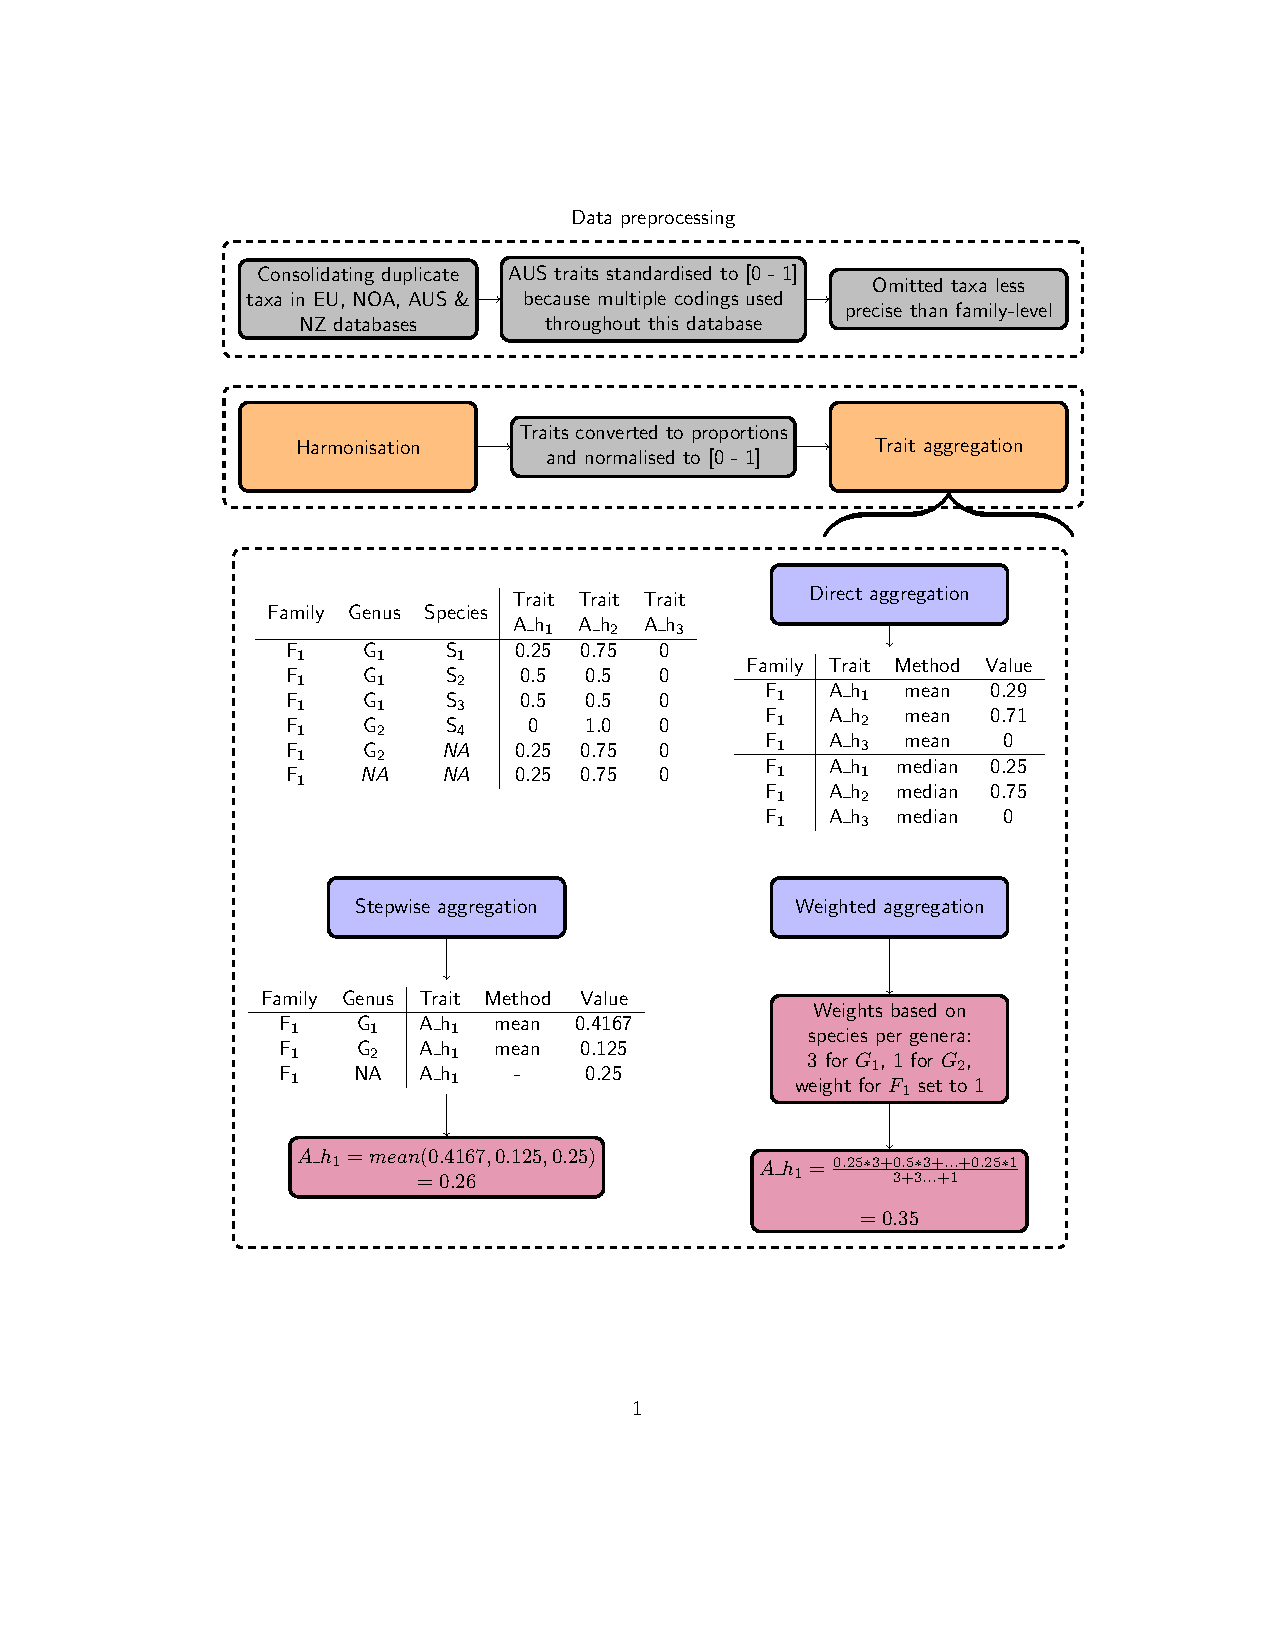
\includegraphics[width=22cm, height=28cm]{Flowchart_methods.pdf}
  \subfile{Flowchart/Flowchart_methods.tex}
  \caption{Data processing steps of the selected traits. Intermediate (grey) and main (orange) steps of data preparation are depicted. The dashed bottom box illustrates the different trait aggregation methods (hypothetical data in the upper left corner). The aggregation methods (purple) and intermediate steps of the aggregation methods (pink) are displayed. Abbreviations: EU, Europe; NOA, North America; AUS, Australia; NZ, New Zealand.}
  \label{fig:data_proc_overview}
\end{figure}

\newpage

%%%%%%%%%%%%%%%%%%%%%%%%%%%%%%%%%%%%%%%%%%%%%%%%%%%%%%%%%%%%%%%%%%%%%%%%%%%%%%%%%%%%%%%%%%%%%%%%%%%%%

\subsection*{Effects of harmonisation and trait aggregation on trait-environment relationship inferences}

To further evaluate the effects of grouping-feature harmonisation and trait aggregation on characterisation of trait–environment relationships, we repeated the analysis of \citet{szocs_effects_2014}, who studied the effects of anthropogenic salinisation on invertebrates in the River Werra in Germany. The River Werra has been subject to effluents from the potash industry since the mid- 20th century, which makes it a useful system for studying the responses of invertebrates and their trait compositions to salinisation (\cite{bathe_biological_2011}). \citet{szocs_effects_2014}  used redundancy analysis (RDA) to compare trait compositions among sites downstream, upstream, and close to salt discharge (transition). Further details about the original study can be found in \citet{szocs_effects_2014}.

We re-analysed the \citet{szocs_effects_2014} study by performing a RDA with harmonised grouping features from the dataset for Europe and with traits that we aggregated to family level with the five aggregation methods described above. We used all 21 grouping features from the original study, but replaced 6 with harmonised grouping features from our European trait dataset, namely: size, feeding mode, locomotion, oviposition, respiration, and voltinism.
We compared the results of the original study’s RDA with the results of the RDA from the harmonised grouping features. Specifically, the trait composition, expressed as community weighted mean (CWM) traits, was ordinated along an electric conductivity gradient. We compared the species scores obtained from the RDA (i.e., the coordinates of the tips of the vectors representing the CWM traits in the bi- or triplots). Following the original study, we used the Mahalanobis distance measure and identified traits associated with higher or lower salinity based on their distance to the ordination axis median. We considered CWM traits with a Mahalanobis distance greater than the 97.5 \%-quantile of the Chi-square distribution (5.02) to have responded to either lower or higher salinity. Additionally, for testing the effect of different aggregation methods on inference about CWM trait–salinisation relationships, we repeated the RDA five times, each with family-level aggregated trait values assigned to corresponding taxa from \citet{szocs_effects_2014}.

%%%%%%%%%%%%%%%%%%%%%%%%%%%%%%%%%%%%%%%%%%%%%%%%%%%%%%%%%%%%%%%%%%%%%%%%%%%%%%%%%%%%%%%%%%%%%%%%%%%%%

\subsection*{Data analysis}

All data processing and RDA analyses were carried out using R (\cite{cite_R}). RDA was computed using the vegan package (\cite{cite_vegan}). Raw data and the R code for data processing and grouping feature harmonisation are located in the Github repository: \url{https://github.com/KunzstLD/Invertebrate_traits}. Scripts and data to reproduce the trait aggregation, comparison of aggregated and assigned traits, and the RDA analysis are located in the Github repository \url{https://github.com/KunzstLD/Trait-aggregation}.

\newpage

%%%%%%%%%%%%%%%%%%%%%%%%%%%%%%%%%%%%%%%%%%%%%%%%%%%%%%%%%%%%%%%%%%%%%%%%%%%%%%%%%%%%%%%%%%%%%%%%%%%%

\section*{Results}

\subsection*{Harmonised trait datasets}

\subsubsection*{Taxonomic coverage of the harmonised trait datasets}

The harmonised European, North American, Australian, and New Zealand trait datasets differed in terms of their taxonomic coverage. The European trait dataset had the largest taxon pool with 4601 taxa (Table \ref{tab:tax_coverage}) followed by the North American dataset (3753 taxa), the Australian dataset (1402 taxa), and the New Zealand dataset with the smallest taxon pool (478 taxa). The European, New Zealand, and North American datasets contained most taxa at the species level, whereas the Australian dataset comprised a similar number of taxa at species and genus level.

\begin{table}[ht]
    \centering
    \caption{Number (Nr.) of taxa per harmonised dataset and per taxonomic level. Numbers in parenthesis show rounded relative frequencies in percent.} 
    \label{tab:tax_coverage}
    \begin{tabular}{lccccc}
    \toprule[.1em]
    Dataset & Taxa (Nr.) & Aquatic insects (Nr.) & Species & Genus & Family \\ 
    \toprule[.1em]
    EU & 4601 & 3942 (86) & 3739 (81) & 704 (15) & 158 (3) \\ 
    NOA & 3753 & 3305 (88) & 2414 (64) & 1163 (31) & 176 (5)  \\ 
    AUS & 1402 & 1016 (72) & 564 (40) & 578 (41) & 260 (19) \\ 
    NZ & 478 & 443 (93) & 404 (85) & 47 (10) & 27 (6) \\ 
    \bottomrule
    \end{tabular}
\end{table}
\begin{minipage}{\linewidth}{\fontsize{8}{10}\selectfont
\centering
Abbreviations: EU, European; NOA, North American; AUS, Australian; NZ, New Zealand.
}
\end{minipage}

%%%%%%%%%%%%%%%%%%%%%%%%%%%%%%%%%%%%%%%%%%%%%%%%%%%%%%%%%%%%%%%%%%%%%%%%%%%%%%%%%%%%%%%%%%%%%%%%%%%%

\subsubsection*{Completeness of trait information}

The numbers of entries with available information for the selected grouping features varied considerably within the harmonised European, North American, and Australian datasets (Table \ref{tab:trait_coverage}). By contrast, the New Zealand dataset contained complete trait information for most of the investigated grouping features (94–100\%).

The amount of entries with available information for the selected grouping features varied strongly for the developed European, North American, and Australian datasets (Table \ref{tab:trait_coverage}). By contrast, the New Zealand dataset contained complete trait information for most of the investigated grouping features (between 94 \% and 100 \%).

\begin{table}[ht]
    \centering
    \caption{Rounded percentage of entries that include 
    information for the individual grouping features
    shown per trait dataset.} 
    \label{tab:trait_coverage}
    \begin{tabular}{lccccccc}
    \toprule[.1em]
    Dataset & Body form & Oviposition & Voltinism & Locomotion & Size & Respiration & Feeding mode \\ 
    \toprule[.1em]
    EU & 8 & 15 & 23 & 36 & 11 & 57 & 76 \\ 
    NOA & 28 & 13 & 47 & 52 & 73 & 44 & 63 \\ 
    AUS & 4 & 46 & 49 & 39 & 75 & 68 & 99 \\ 
    NZ & 100 & 94 & 100 & 99 & 100 & 100 & 99 \\ 
    \bottomrule
    \end{tabular}
\end{table}
\begin{minipage}{\linewidth}{\fontsize{8}{10}\selectfont
\centering
Abbreviations: EU, European; NOA, North American; AUS, Australian; NZ, New Zealand.
}
\end{minipage}

\newpage

%%%%%%%%%%%%%%%%%%%%%%%%%%%%%%%%%%%%%%%%%%%%%%%%%%%%%%%%%%%%%%%%%%%%%%%%%%%%%%%%%%%%%%%%%%%%%%%%%%%%

\subsubsection*{Discrepancies in invertebrate trait definitions across databases}

Definitions of grouping features and traits varied in their level of detail in the investigated trait databases. The freshwaterecology.info, Tachet, and CONUS databases provided more detailed descriptions of trait information than the Vieira and New Zealand databases provided. The Australian trait database (\cite{kefford_integrated_2020}) was a collection of seven specific trait datasets; thus, grouping features occurred multiple times with varying differentiation into traits. Depending on the dataset, trait information was described with more or less detail.

The definitions of grouping features also varied across databases in their differentiation into traits and in their focus, both which can lead to discrepancies in trait definitions. We provide a summary of discrepancies in trait definitions in the appendix (Table \ref{stab:trait_definitions}). Varying levels of differentiation among the trait databases were present in all investigated grouping features (Table \ref{tab:trait_databases_coding_differentiation} and Table \ref{stab:trait_definitions}).

For example, for the grouping feature feeding mode, discrepancies arose because traits were assigned in different ways. The Tachet database defined predators as carvers, engulfers, and swallowers. By contrast, the CONUS database defined predators as engulfers and carnivorous piercers. In turn, the Tachet database defined piercers as a separate trait encompassing both herbivorous and carnivorous piercers. Furthermore, the focus in the freshwaterecology.info database for feeding mode was primarily on the food source of a species (except for filterers), whereas the other databases focused on the strategies of food acquisition. For example, the freshwaterecology.info database defined predator as "eating from prey", and the other databases used the mouthpart morphology as basis for their definitions. The Tachet database captured the food source in an additional grouping feature. Locomotion definitions also differed in focus among databases. The New Zealand and freshwaterecology.info databases described locomotion as an organism’s way of movement, Tachet as substrate relation and locomotion, Vieira as how organisms deal with flow, Australia as attachment, and CONUS included not only the method of movement but also the location of movement. Similarly, databases differed in their focus for reproduction traits. In the freshwaterecology.info and Tachet databases, reproduction was captured in one grouping feature and was defined as location of oviposit clutches and mode of reproduction. The Vieira database provided information on the oviposition location but not on reproductive behaviour. The Australian database reported grouping features for reproductive behaviour but also on oviposition location separately. The New Zealand database distinguished three grouping features related to reproduction: reproductive technique, oviposition location (e.g. water surface, terrestrial), and egg/egg mass (e.g. free, cemented).

Trait affinity scores also varied among the databases and were described by varying coding methods (e.g., binary, fuzzy, continuous). In the freshwaterecology.info and Australian databases a combination of coding methods is used, whereas in the Tachet and New Zealand databases exclusively fuzzy coding is used. The Vieira and CONUS databases contained categorical grouping features that can be converted into binary trait affinities (Table \ref{tab:trait_databases_coding_differentiation}).


\begin{landscape}
\begin{longtable}{m{2.3cm}|m{3cm}|m{1.8cm}|m{1.4cm}|m{1.4cm}|m{4.1cm}|m{2cm}}
\caption{Number of traits per grouping feature and type of coding of the traits for the grouping features used in this study per database. Oviposition location was used for the New Zealand database.}
\endfirsthead
\toprule[.1em]
\label{tab:trait_databases_coding_differentiation}
\specialcell{Grouping \\ feature} & \specialcell{freshwater- \\ ecology.info} & Tachet & CONUS & Vieira & Australia & New Zealand \\
\toprule[.1em]
Feeding Mode & \begin{tabular}[c]{@{}l@{}}10 traits; \\ 10 point assginment \\ system\end{tabular}       & \begin{tabular}[c]{@{}l@{}}7 traits; \\ fuzzy {[}0 - 3{]}\end{tabular} & \begin{tabular}[c]{@{}l@{}}6 traits; \\ binary\end{tabular}   & \begin{tabular}[c]{@{}l@{}}8 traits; \\ binary\end{tabular}  & \begin{tabular}[c]{@{}l@{}}16 traits$^{\dagger}$; \\ binary, proportional {[}0 - 1{]}, \\ fuzzy {[}0 - 3{]}\end{tabular} & \begin{tabular}[c]{@{}l@{}}6 traits; \\ fuzzy {[}0 - 3{]}\end{tabular} \\
\midrule
Voltinism                                                           & \begin{tabular}[c]{@{}l@{}}6 traits; \\ single category \\ assignment system\end{tabular} & \begin{tabular}[c]{@{}l@{}}3 traits; \\ fuzzy {[}0 - 3{]}\end{tabular} & \begin{tabular}[c]{@{}l@{}}3 traits;\\ binary\end{tabular}    & \begin{tabular}[c]{@{}l@{}}3 traits; \\ binary\end{tabular}  & \begin{tabular}[c]{@{}l@{}}7 traits; \\ binary, proportional {[}0 - 1{]}, \\ fuzzy {[}0 - 3{]}\end{tabular}  & \begin{tabular}[c]{@{}l@{}}3 traits; \\ fuzzy {[}0 - 3{]}\end{tabular} \\
\midrule
Locomotion                                                          & \begin{tabular}[c]{@{}l@{}}6 traits; \\ 10 point assignment \\ system\end{tabular}        & \begin{tabular}[c]{@{}l@{}}8 traits; \\ fuzzy {[}0 - 5{]}\end{tabular} & \begin{tabular}[c]{@{}l@{}}10 traits; \\ binary\end{tabular}  & \begin{tabular}[c]{@{}l@{}}9 traits; \\ binary\end{tabular}  & \begin{tabular}[c]{@{}l@{}}9 traits; \\ binary, fuzzy  {[}0 - 3{]}\end{tabular}                              & \begin{tabular}[c]{@{}l@{}}4 traits; \\ fuzzy {[}0 - 3{]}\end{tabular} \\
\midrule
Respiration                                                         & \begin{tabular}[c]{@{}l@{}}7 traits; \\ binary\end{tabular}                               & \begin{tabular}[c]{@{}l@{}}5 traits; \\ fuzzy {[}0 - 3{]}\end{tabular} & \begin{tabular}[c]{@{}l@{}}3 traits;  \\ binary\end{tabular}  & \begin{tabular}[c]{@{}l@{}}8 traits; \\ binary\end{tabular}  & \begin{tabular}[c]{@{}l@{}}10 traits; \\ binary, proportional {[}0 - 1{]}, \\ fuzzy {[}0 - 3{]}\end{tabular} & \begin{tabular}[c]{@{}l@{}}4 traits; \\ fuzzy {[}0 - 3{]}\end{tabular} \\
\midrule
\begin{tabular}[c]{@{}l@{}}Reproduction/\\ Oviposition\end{tabular} & \begin{tabular}[c]{@{}l@{}}9 traits; \\ binary\end{tabular}                               & \begin{tabular}[c]{@{}l@{}}8 traits; \\ fuzzy {[}0 - 3{]}\end{tabular} & \begin{tabular}[c]{@{}l@{}}10 traits;  \\ binary\end{tabular} & \begin{tabular}[c]{@{}l@{}}10 traits; \\ binary\end{tabular} & \begin{tabular}[c]{@{}l@{}}13 traits$^{\ddagger}$; \\ binary\end{tabular}                                                 & \begin{tabular}[c]{@{}l@{}}4 traits; \\ fuzzy {[}0 - 3{]}\end{tabular} \\
\midrule
Size                                                                & -                                                                                         & \begin{tabular}[c]{@{}l@{}}7 traits;\\ fuzzy {[}0 - 3{]}\end{tabular}  & \begin{tabular}[c]{@{}l@{}}3 traits; \\ binary\end{tabular}   & \begin{tabular}[c]{@{}l@{}}3 traits; \\ binary\end{tabular}  & \begin{tabular}[c]{@{}l@{}}9 traits; \\ binary, continuous, \\ \\ fuzzy {[}0 - 3{]}\end{tabular}             & \begin{tabular}[c]{@{}l@{}}5 traits; \\ fuzzy {[}0 - 3{]}\end{tabular} \\
\midrule
Body Form                                                           & -                                                                                         & -                                                                      & -                                                             & \begin{tabular}[c]{@{}l@{}}4 traits; \\ binary\end{tabular}  & \begin{tabular}[c]{@{}l@{}}4 traits; \\ fuzzy {[}0 - 3{]}\end{tabular}                                       & \begin{tabular}[c]{@{}l@{}}4 traits; \\ fuzzy {[}0 - 3{]}\end{tabular} \\
\bottomrule
\end{longtable}
\begin{minipage}{\linewidth}\small
      $\dagger$ Some of the feeding mode traits used in the Australian database were similar (e.g. trait \textit{Shredder}, \textit{Shredder, Detrivore}, and \textit{Collector, Shredder}).
      \newline
      $\ddagger$ Not all traits were considered because trait information was partly presented as comments to describe other traits or due to incomplete information.
  \end{minipage}
\end{landscape}


%%%%%%%%%%%%%%%%%%%%%%%%%%%%%%%%%%%%%%%%%%%%%%%%%%%%%%%%%%%%%%%%%%%%%%%%%%%%%%%%%%%%%%%%%%%%%%%%%%%%

\subsection*{Comparing aggregation methods} 

\subsubsection*{Comparison of family-level aggregated traits with family-level assigned traits}
\label{sec:diff_trait_agg_chessman}

The comparison of family-level aggregated trait affinities with those assigned by experts for the Australian and North American databases showed that aggregation method (median or mean) had a greater effect than the overall approach (direct, stepwise, or weighted by the number of species) in whether trait affinities differed from those assigned by experts.

The percentage of differing cases of aggregated versus assigned trait affinities varied by method between 16.2 and 22.9 \% for the Australian dataset and between 15.3 and 47 \% for the North American dataset (Table \ref{tab:summary_stat_aggr_vs_fam_assigned}). In general, median aggregation methods yielded fewer cases with differences compared with mean aggregation methods. However, median aggregation methods produced, on average, greater absolute differences for both datasets. Standard deviations of absolute differences were similar for all tested aggregation methods. Maximum differences of 1 (i.e., the maximum possible difference) occurred for all investigated grouping features in both datasets (Figure \ref{fig:diff_aggr_traits_combined}).

\begin{table}[H]
  \centering
  \caption{Percentage of differing cases, minimum, maximum, mean, and standard deviation of absolute differences between trait affinities assigned at family level by experts and aggregated trait affinities from five different aggregation methods.}
  \label{tab:summary_stat_aggr_vs_fam_assigned}
  \begin{tabular}{ll|ccccc}
  \toprule[.1em]
  Database & \specialcell{Comparison to\\ traits at family level} & \specialcell{Differing \\ cases [\%]} & \specialcell{Min. \\ differences} & \specialcell{Max. \\ differences} & \specialcell{Mean abs. \\ differences} & \specialcell{SD abs. \\ differences} \\ 
  \toprule[.1em]
  \multirow{4}{*}{\specialcell{Australia}} & \specialcell{\textit{direct\_agg (median)}} & 16.53 & 0.01 & 1.00 & 0.45 & 0.27 \\ 
  & \specialcell{\textit{direct\_agg (mean)}} & 23.24 & $< 0.01$ & 0.99 & 0.34 & 0.23 \\ 
  & \specialcell{\textit{stepwise\_agg (median)}} & 17.90 & 0.01 & 1.00 & 0.42 & 0.26 \\ 
  & \specialcell{\textit{stepwise\_agg (mean)}} & 23.24 & $< 0.01$ & 0.99 & 0.33 & 0.22 \\ 
  & \specialcell{\textit{weighted\_agg}} & 23.24 & $< 0.01$ & 1.00 & 0.34 & 0.24 \\ 
  \midrule
  \multirow{4}{*}{\specialcell{North America}} & \specialcell{\textit{direct\_agg (median)}} & 15.33 & 0.17 & 1.00 & 0.70 & 0.26 \\ 
  & \specialcell{\textit{direct\_agg (mean)}} & 47.00 & $< 0.01$ & 1.00 & 0.30 & 0.26 \\ 
  & \specialcell{\textit{stepwise\_agg (median)}} & 18.00 & 0.08 & 1.00 & 0.63 & 0.28 \\ 
  & \specialcell{\textit{stepwise\_agg (mean)}} & 47.00 & $< 0.01$ & 1.00 & 0.30 & 0.27 \\ 
  & \specialcell{\textit{weighted\_agg}} & 47.00 & $< 0.01$ & 1.00 & 0.31 & 0.28 \\ 
  \bottomrule
  \end{tabular}
\end{table}
\begin{minipage}{\linewidth}{\fontsize{8}{10}\selectfont
  \centering
  Abbreviations: Min., Minimum; Max., Maximum; abs., absolute; SD, Standard deviation.
  }
  \end{minipage}


\newpage

\begin{figure}[H]
  \centering
  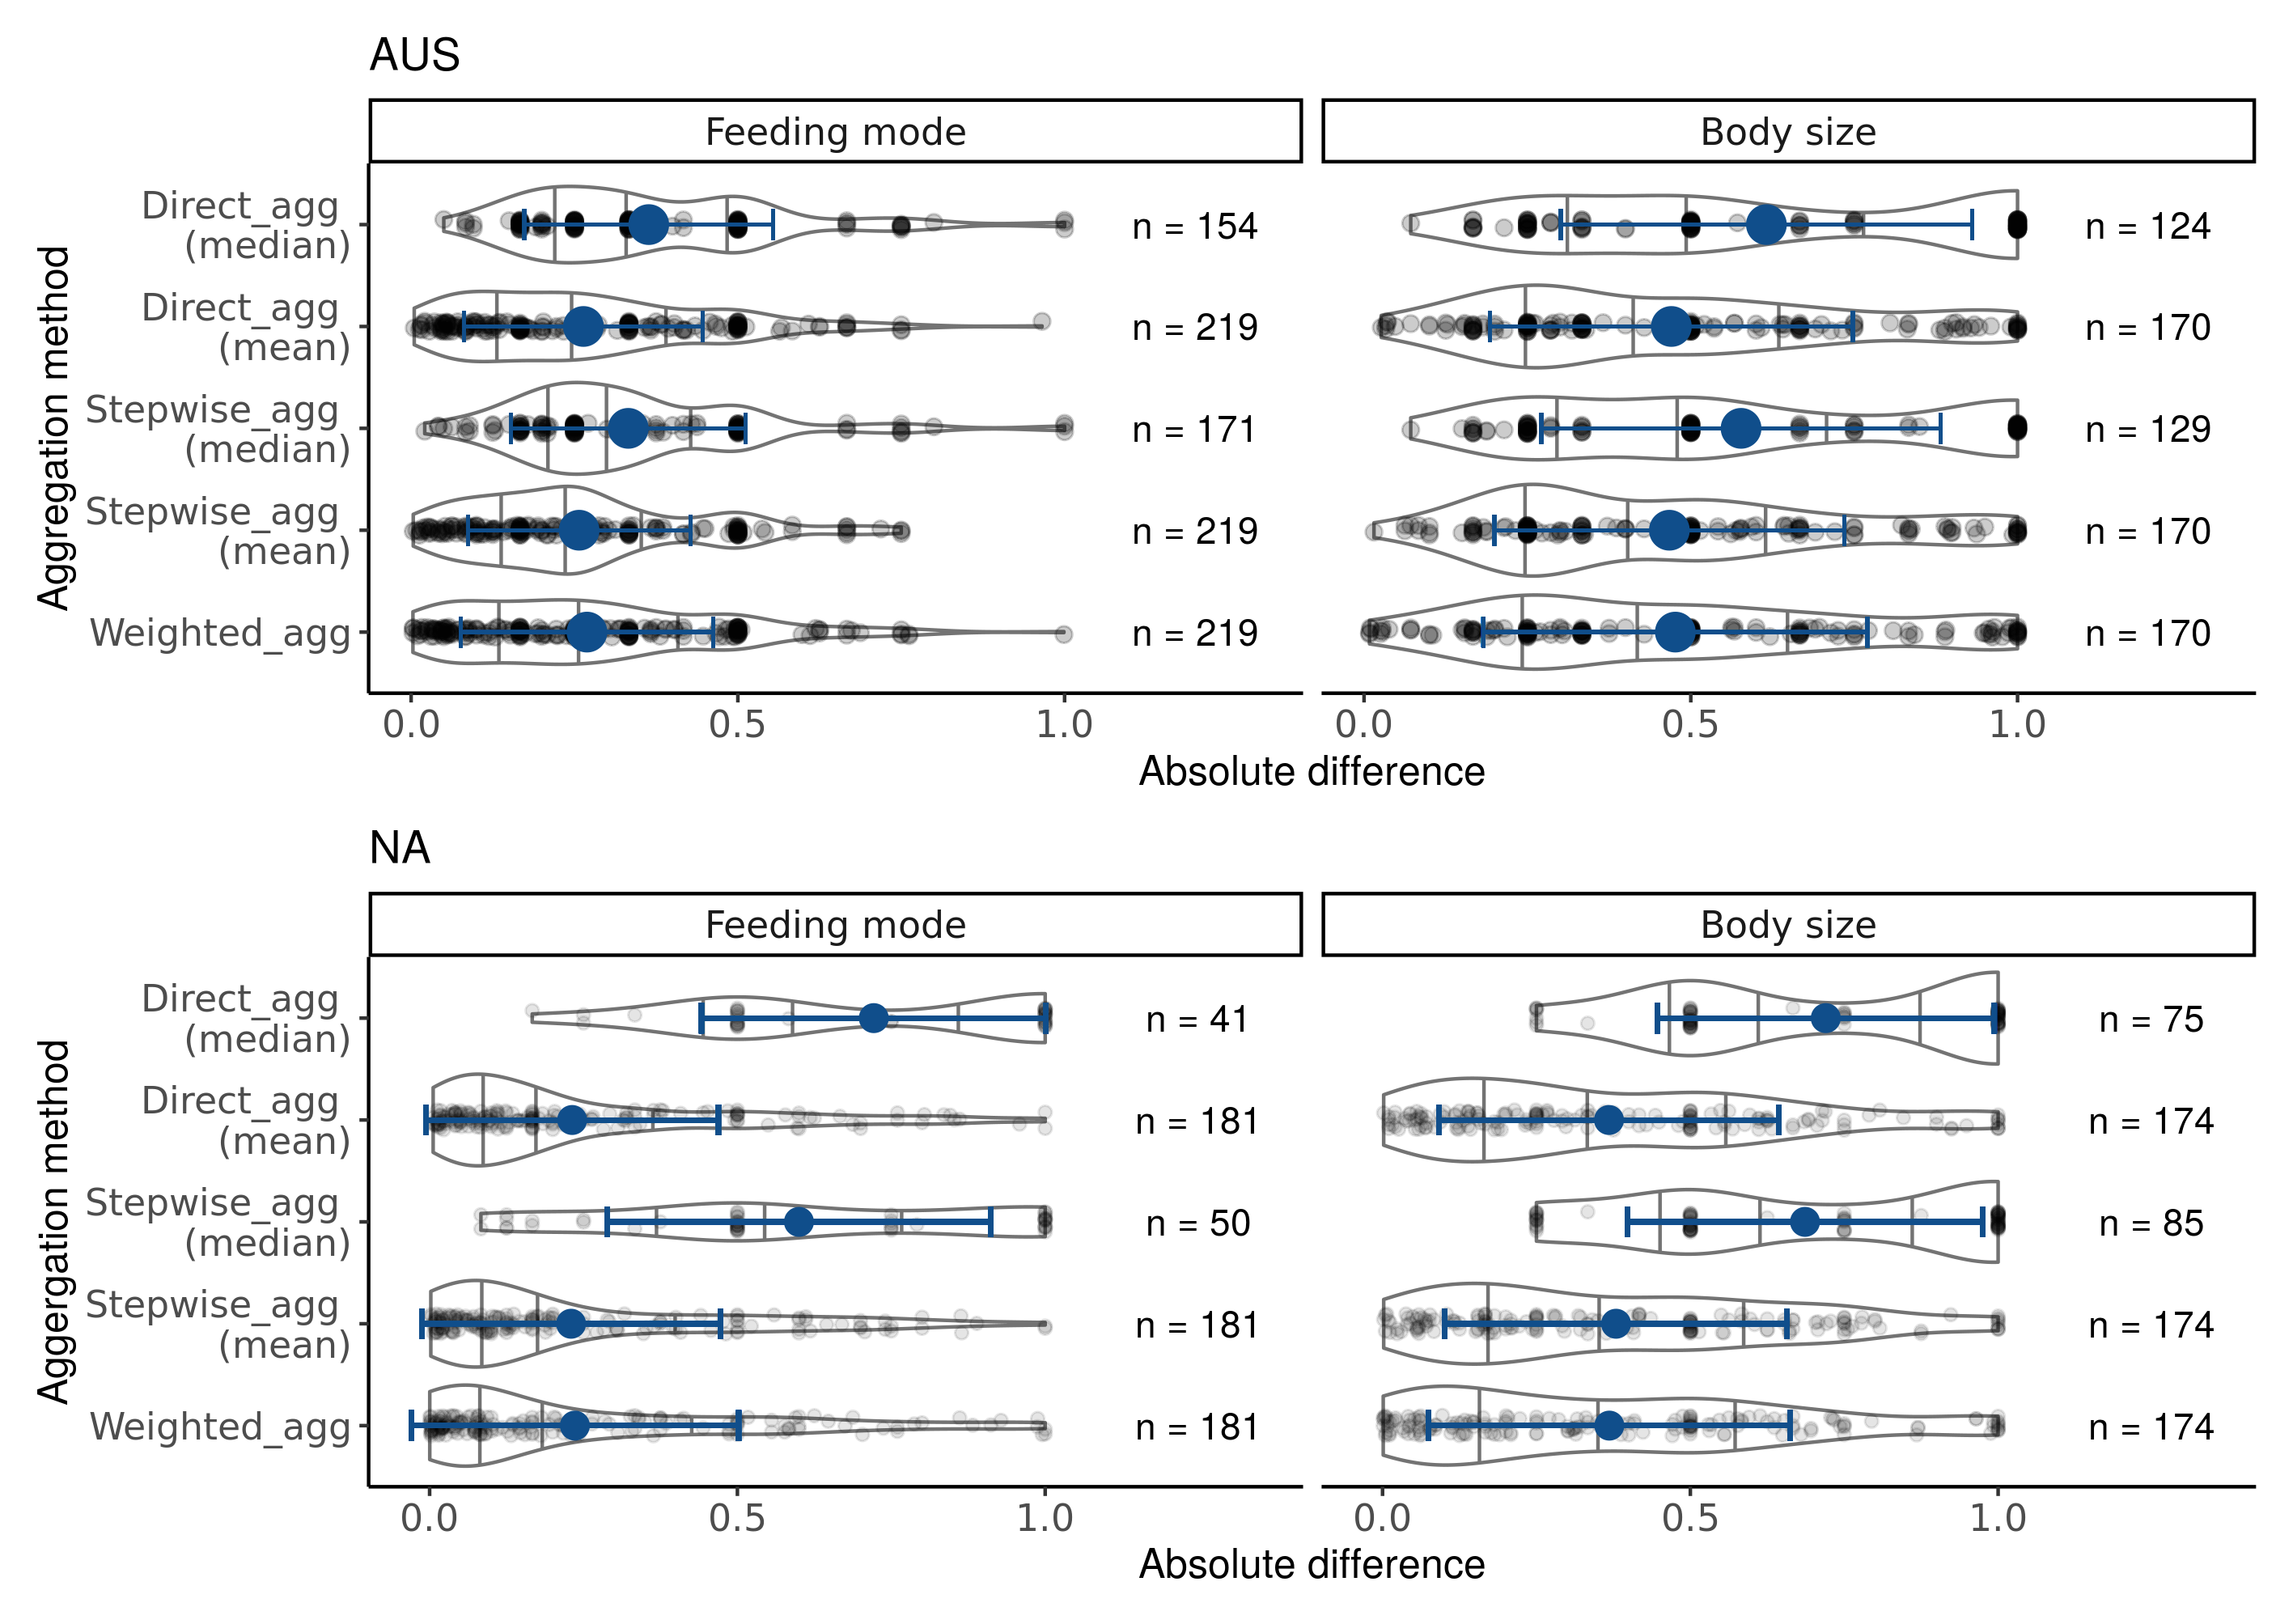
\includegraphics[width=16.5cm, height=12cm]{Deviances_trait_agg_combined.png}
  \caption{Cases (factor combination of investigated families and traits) where differences occurred between aggregated traits and expert assigned traits at family level for the Australian and North American dataset. Violin plots - mirrored density plots - show the density of the absolute trait affinity differences for the grouping features feeding mode and body size. Results for the North American dataset for the grouping features locomotion, respiration, and voltinism are shown in the supporting information (Figure \ref{fig:diff_aggr_traits_pyne}). Absolute differences in trait affinities are depicted as grey dots. \textit{n} denotes the number of cases per comparison where differences occurred. The blue dot indicates the mean of absolute differences, and the error bars show the standard deviation. The grey vertical lines show the 25\textsuperscript{th}, 50\textsuperscript{th} and 75\textsuperscript{th} quantiles of the density estimate. Abbreviations: AUS, Australia; NOA, North America.}
  \label{fig:diff_aggr_traits_combined}
\end{figure}

\newpage 


\subsubsection*{Comparison of aggregation methods with varying taxonomic hierarchies and trait variability}

Our simulation results showed that both taxonomic hierarchical structure and trait variability affected aggregated trait affinities, although only to a small degree, and that aggregation method mattered in terms of the ranges of trait affinities produced over simulation replicates. The effect of taxonomic hierarchy differed across aggregation methods, but, as we expected, the produced range of trait affinities increased with increasing trait variability for all aggregation methods (Figure \ref{fig:overview_sim_results}). % Ben would add: % as indicated by the increasing range of the boxes and wiskers with increasing standard deviation. 

Taxonomic hierarchical structure appeared to influence the outcomes of the different aggregation methods. For the \textit{sim\_base} scenario (equal numbers of genera and species), the mean and weighted aggregation methods yielded similar ranges of aggregated trait affinities within each level of trait variability, and the median aggregation methods consistently produced greater ranges of aggregated trait affinities than the other methods. The largest ranges were produced by the \textit{stepwise\_agg \textsubscript{median}} method. For the more complex taxonomic hierarchical structures, \textit{sim\_extreme} (one genus with a much larger number of species than the other four) and \textit{sim\_variation} (all genera with a different number of species), the \textit{stepwise\_agg \textsubscript{median}} method still produced the largest ranges of trait affinities for most levels of trait variability (and \textit{direct\_agg\textsubscript{mean}} produced the narrowest ranges for most levels of trait variability), but there was much less consistency in the ranges of trait affinities for all aggregation methods (i.e., the ranges were different among all aggregation methods).

Although trait aggregation methods were affected by taxonomic hierarchical structure and trait variability to some degree, in most simulated datasets, the different aggregation methods resulted in similar trait affinities. Only 1.42 \%, or 213 out of 15.000 total comparisons (3 scenarios $*$ 5 levels of trait variability $*$ 10 unique comparisons of trait aggregation methods $*$ 100 replicates) showed a difference equal or greater than an absolute trait affinity of 0.1. Most  (83.5 \%) of these differences occurred in the \textit{sim\_extreme} scenario and were found between the aggregation methods \textit{direct\_agg\textsubscript{mean}} and \textit{stepwise\_agg\textsubscript{median}}, \textit{direct\_agg\textsubscript{median}} and \textit{stepwise\_agg\textsubscript{median}}, and \textit{stepwise\_agg\textsubscript{median}} and \textit{weighted\_agg} (Figure \ref{fig:sim_indv_runs}). 

\begin{figure}[H]
  \centering
  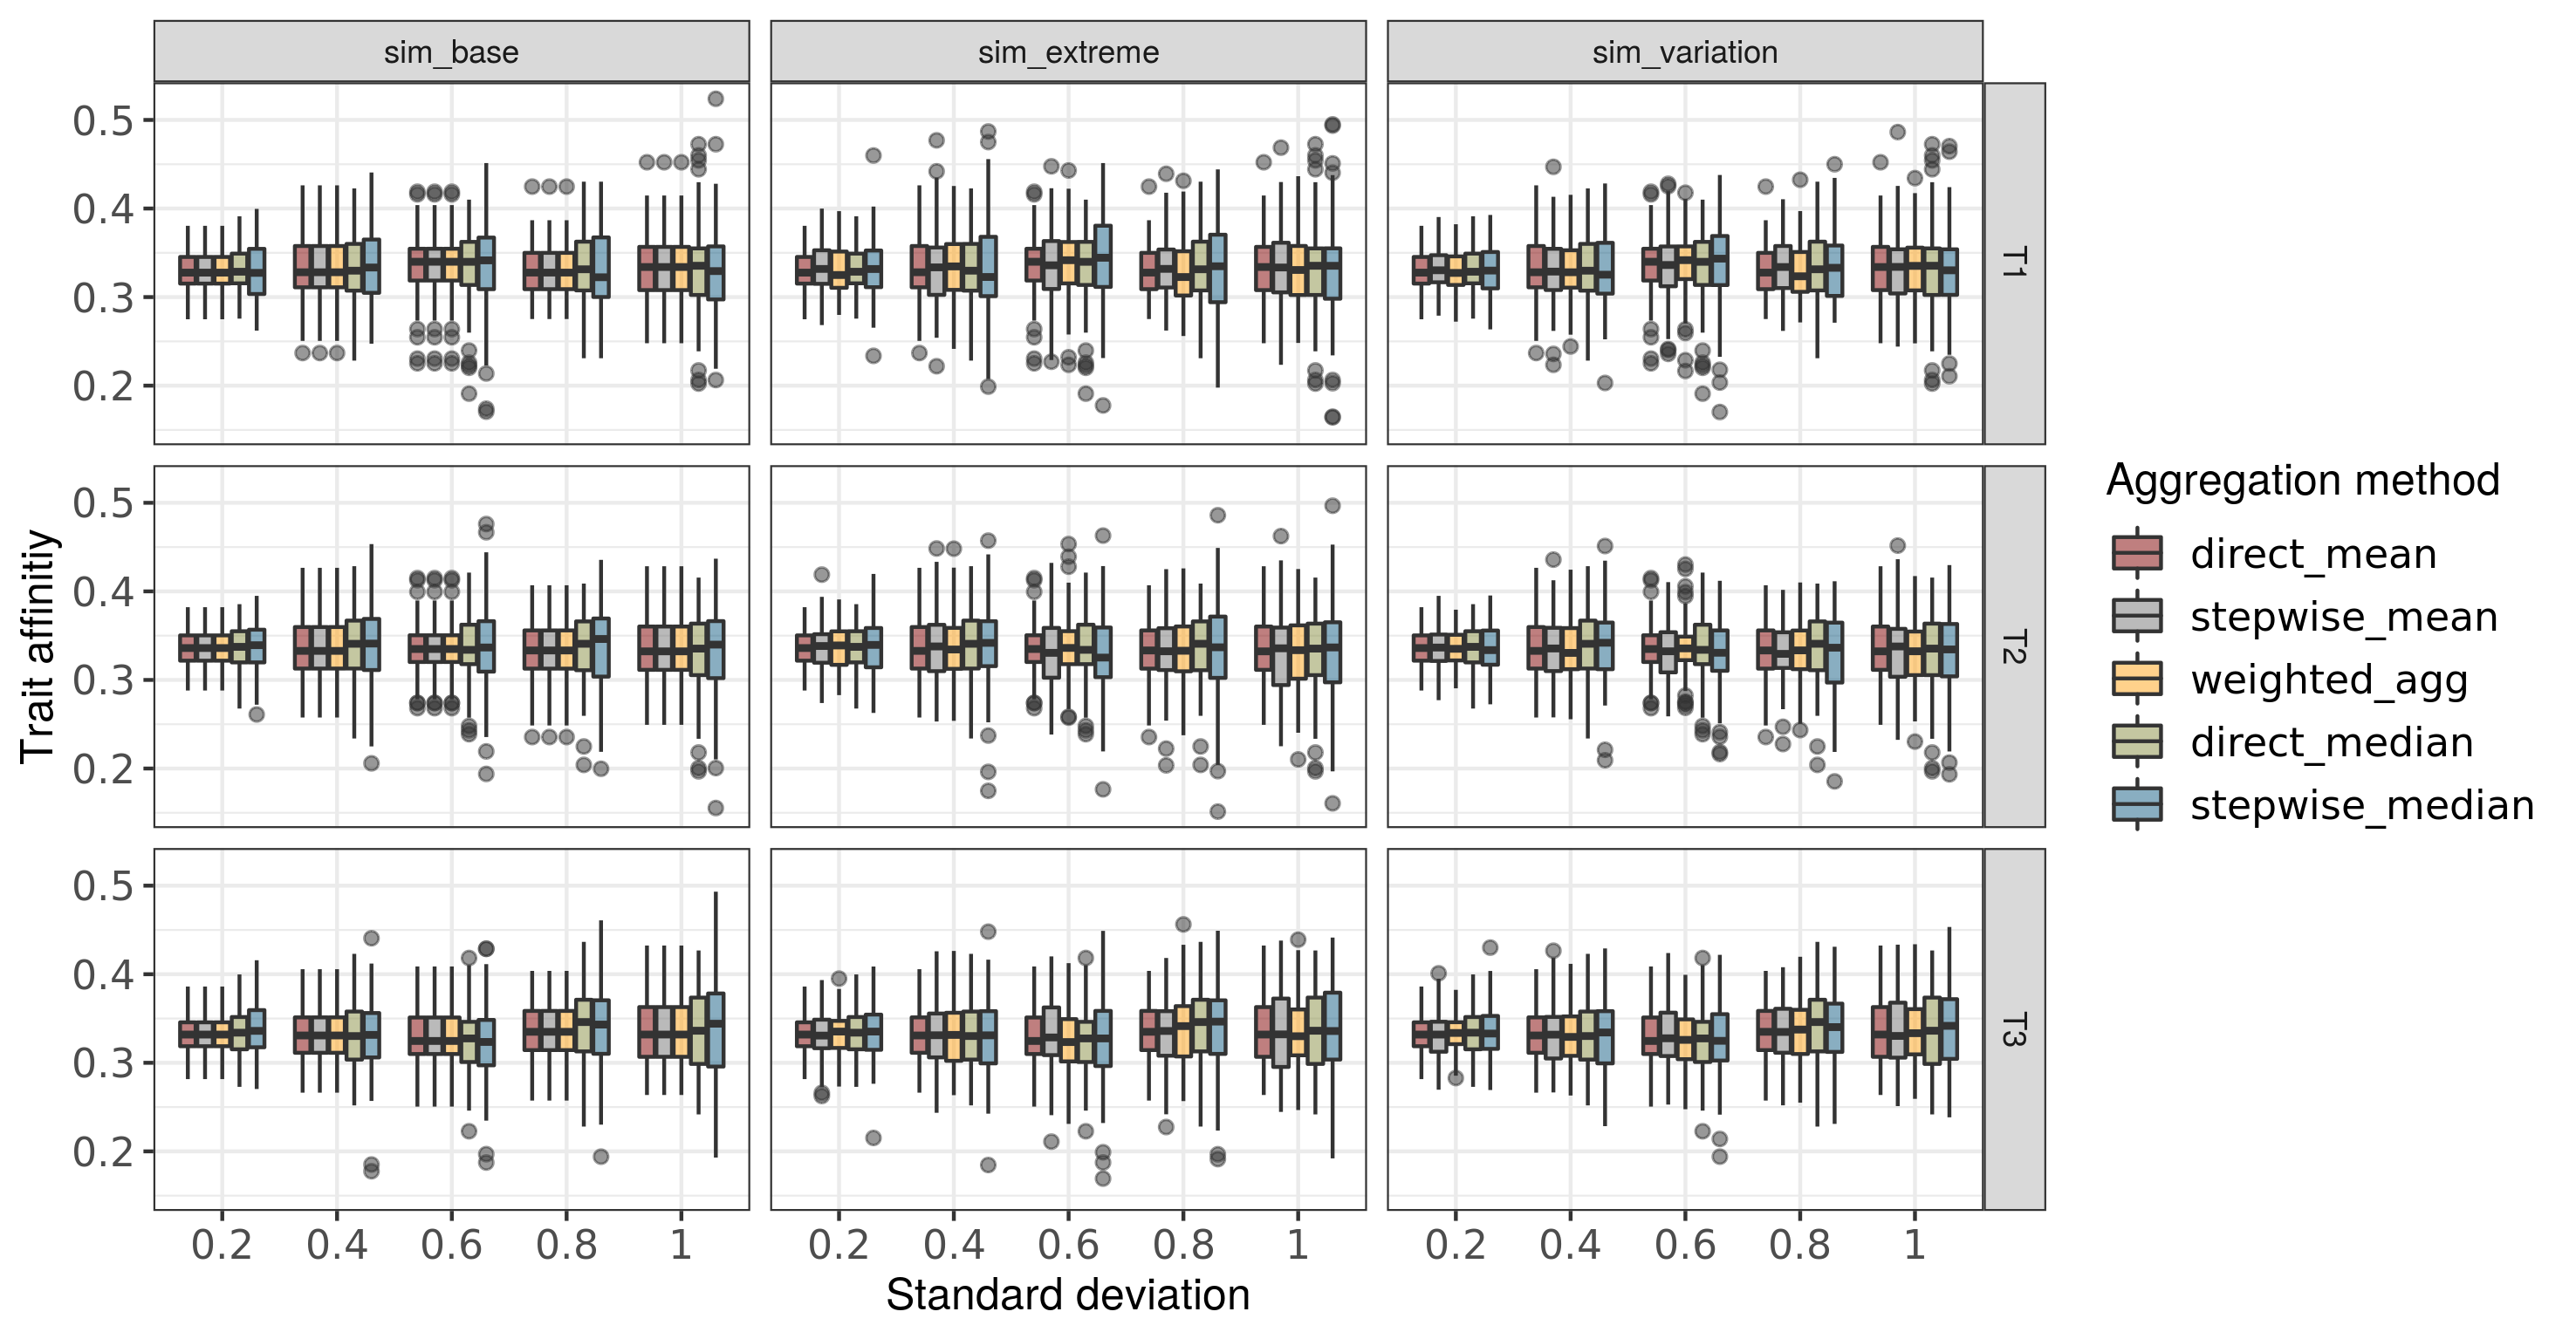
\includegraphics[width=16.5cm, height=10cm]{Overview_sim_results.png}
  \caption{Ranges of aggregated trait affinities for the three examples of taxonomic hierarchies and simulated levels of trait variability. Shown are the results only for one simulated trait (T1). Similar results were obtained for the other simulated traits (Figure \ref{fig:overview_sim_results_T2_T3}). Boxplots depict results for 100 replicated simulations of each trait aggregation method. The boxplot depicts the median and encompasses the 25\textsuperscript{th} and 75\textsuperscript{th} percentile. Horizontal black lines depict the median. Whiskers extend to the largest and smallest value respectively no further than 1.5 $*$ the inter-quartile range. Outliers beyond the end of the whiskers are plotted as grey dots. Trait aggregation methods are in order of least to greatest produced ranges to improve visual inspection.}
  \label{fig:overview_sim_results}
\end{figure}

\begin{figure}[H]
  \centering
  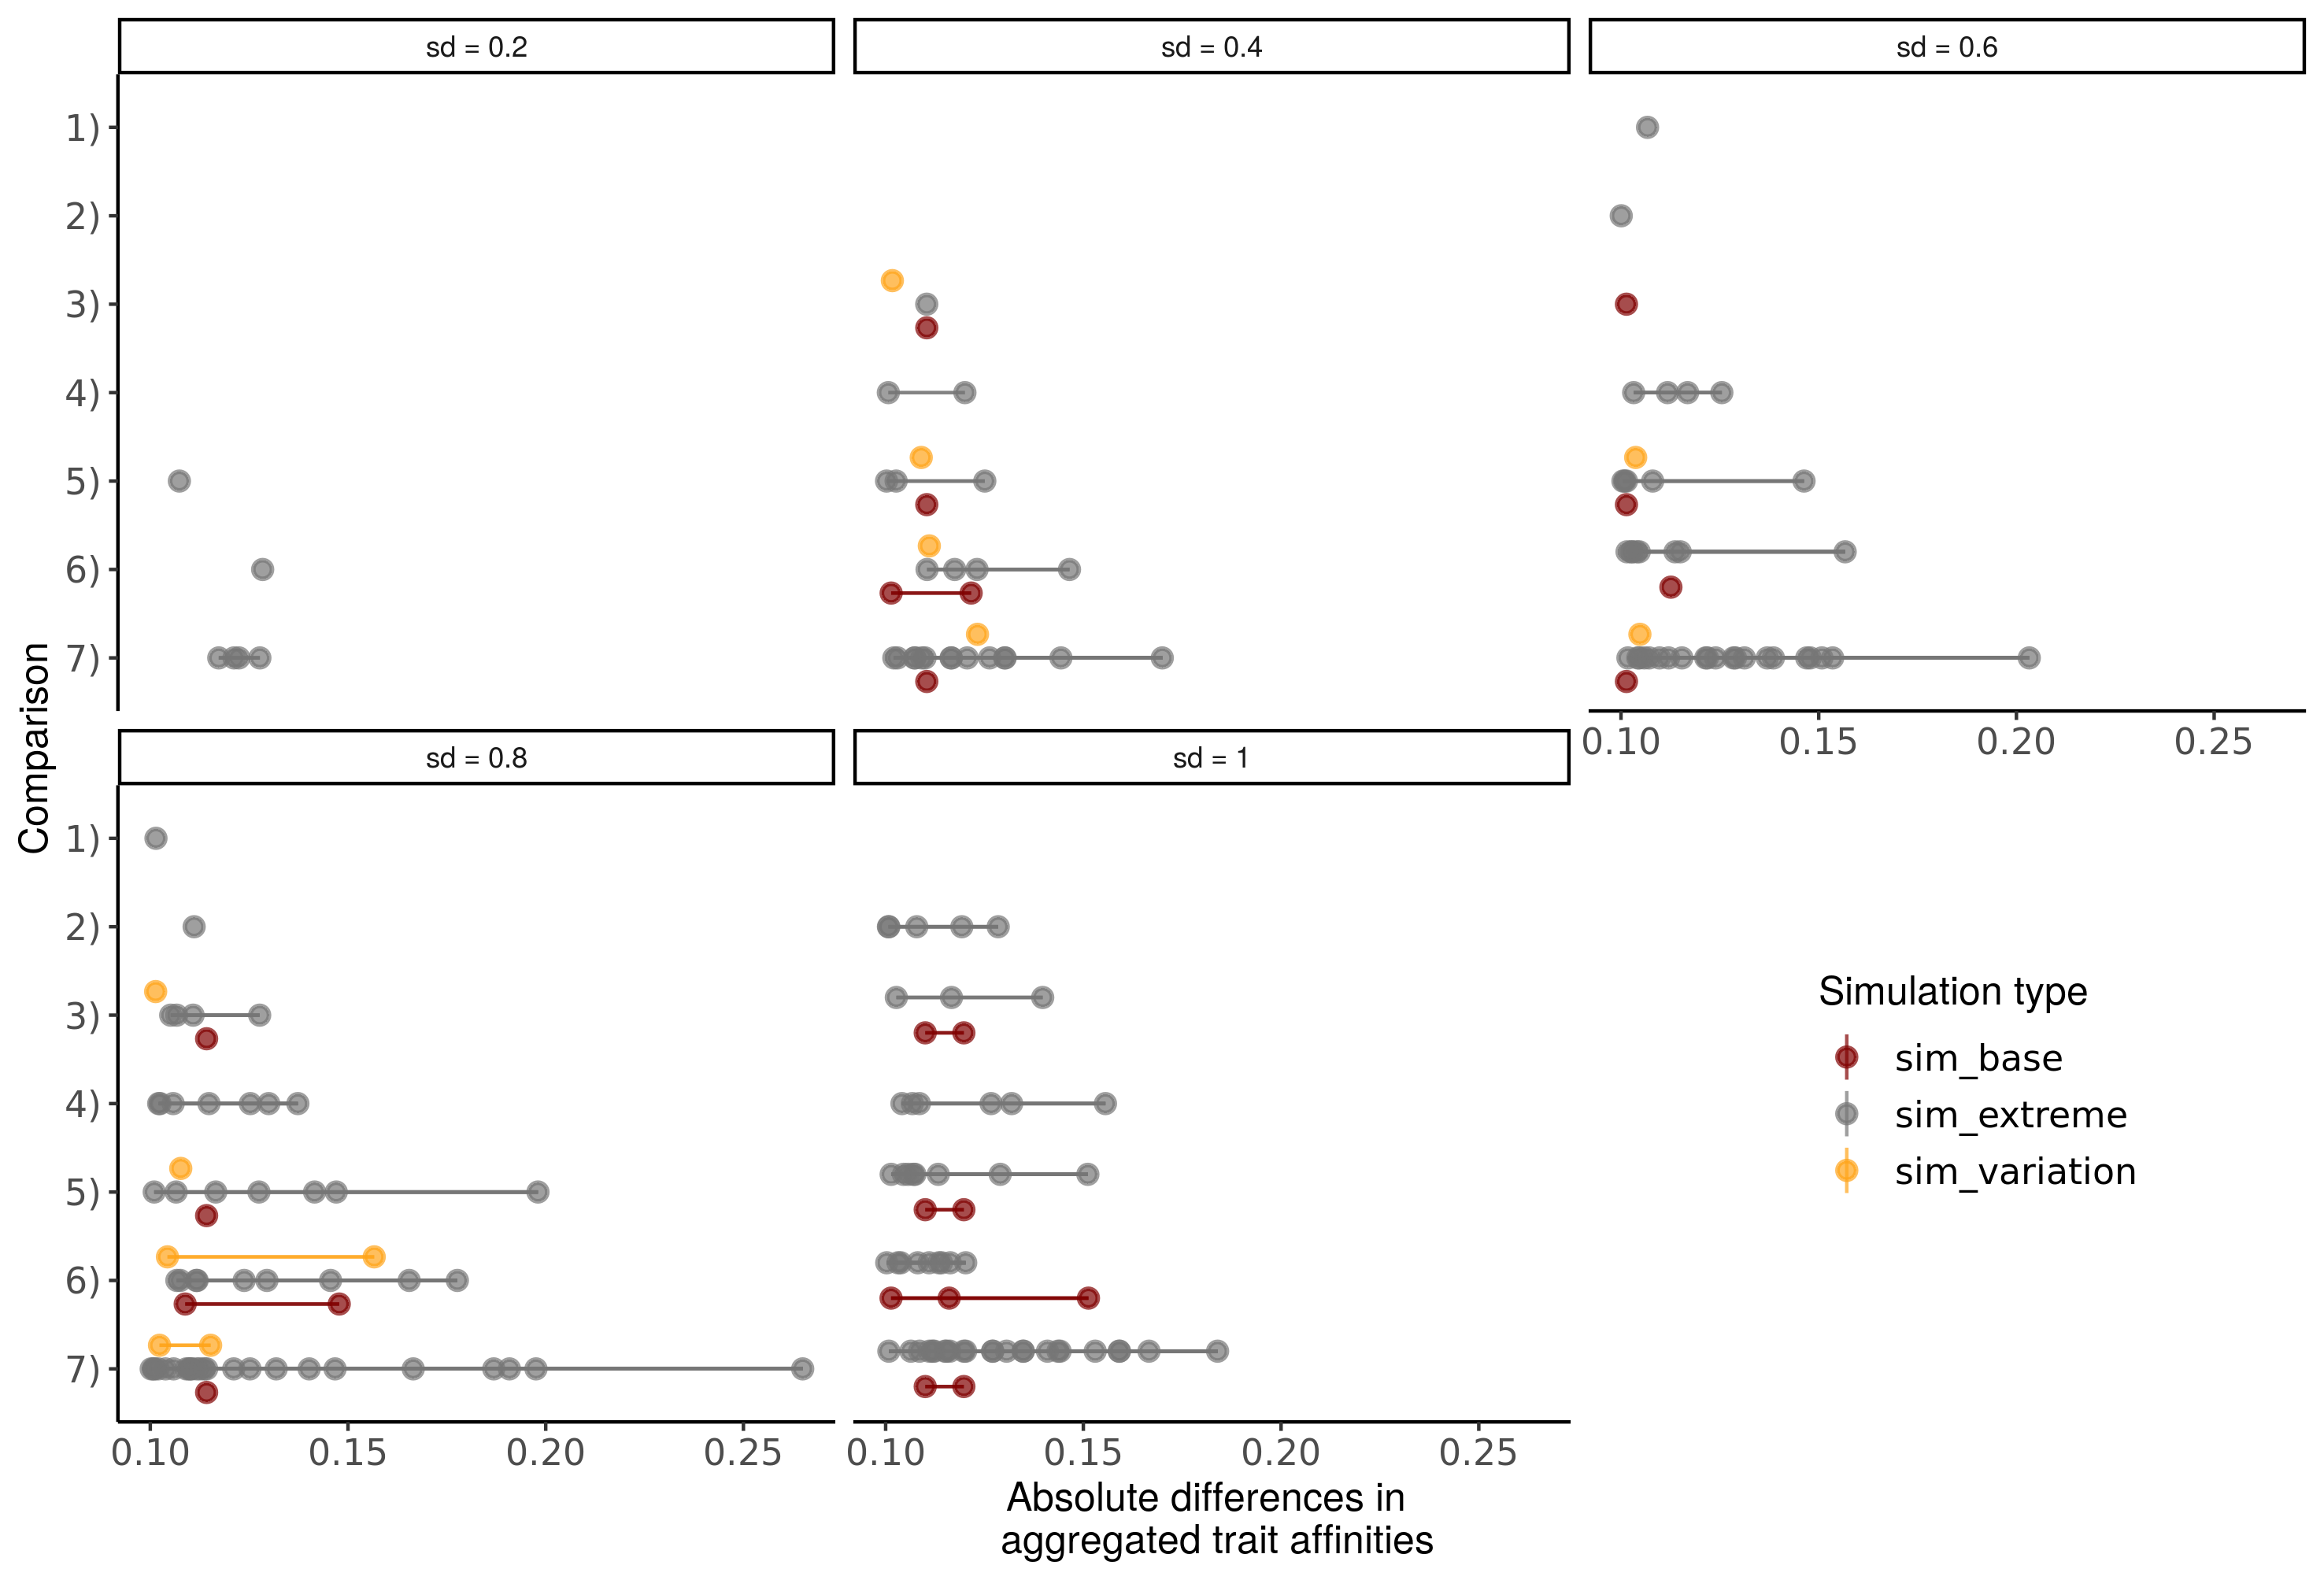
\includegraphics[width=16.5cm, height=10cm]{Diffs_indiv_runs_sim.png}
  \caption{Comparison between the aggregated trait affinities produced by the different trait aggregation methods for every simulated dataset across all 3 simulated traits (5,000 comparisons per taxonomic hierarchy scenario). Results are shown for different levels of trait variability which is represented by the standard deviation (SD) of the simulated traits. Dots depict comparisons where absolute differences between aggregated trait affinities were greater than 0.1. Overall, there are 10 possible unique comparisons of which 7 produced absolute differences greater than 0.1. \newline
  Comparisons: \newline
  1) \textit{direct\_agg (median)} - \textit{stepwise\_agg (mean)} \newline
  2) \textit{direct\_agg (median)} - \textit{weighted\_agg} \newline
  3) \textit{stepwise\_agg (mean)} - \textit{stepwise\_agg (median)} \newline
  4) \textit{stepwise\_agg (mean)} - \textit{weighted\_agg} \newline  
  5) \textit{direct\_agg (mean)} - \textit{stepwise\_agg (median)} \newline
  6) \textit{direct\_agg (median)} - \textit{stepwise\_agg (median)} \newline
  7) \textit{stepwise\_agg (median)} - \textit{weighted\_agg} \newline
  }
  \label{fig:sim_indv_runs}
\end{figure}

\newpage

%%%%%%%%%%%%%%%%%%%%%%%%%%%%%%%%%%%%%%%%%%%%%%%%%%%%%%%%%%%%%%%%%%%%%%%%%%%%%%%%%%%%%%%%%%%%%%%%%%%%

\subsection*{Effects of harmonisation and trait aggregation on trait-environment relationships}

Our re-analysis of the \citet{szocs_effects_2014} study on the effects of salinisation on invertebrate traits showed that the use of harmonised and aggregated trait data may be useful for ecological studies on trait–environment relationships. Overall, harmonised trait data and all aggregation methods produced similar distributions of RDA species scores (\ref{fig:violin_plot_species_sc}) compared with the original analysis, and they resulted in similar, but fewer, traits that distinguished upstream and downstream sites than the original analysis (Figures \ref{fig:violin_plot_species_sc} and \ref{fig:boxplot_scores_on_constrained_axis}).

RDA using harmonised, but not aggregated, grouping features identified some, but not all, of the same traits that were identified by the original analysis (Figures \ref{fig:violin_plot_species_sc} and \ref{fig:boxplot_scores_on_constrained_axis}). The original RDA in \citet{szocs_effects_2014} indicated that downstream sites (higher salinity) were characterised by the traits: ovoviviparity, multivoltinism, long life-cycle duration ($> 1$ year), shredder, and gill respiration, whereas RDA with the harmonised data identified the first three traits but did not include shredder or gill respiration traits. The original RDA indicated that upstream sites (lower salinity) were characterised by the traits: univoltinism, oviposition in clutches, and short life-cycle duration ($< 1$ year), and RDA with the harmonised data characterised upstream sites by univoltine taxa with short life-cycle durations that lay their eggs in an aquatic environment (aquatic eggs). This difference in oviposition trait is not substantial because the trait aquatic eggs of the harmonised grouping feature oviposition was derived by combining the trait oviposition in clutches and other related traits (Table \ref{tab:traits_harmonisation}).

RDA using harmonised traits that were aggregated to family level also produced results similar to the original analysis but with fewer traits distinguishing upstream and downstream sites (Figures \ref{fig:violin_plot_species_sc} and \ref{fig:boxplot_scores_on_constrained_axis}). The \textit{direct\_agg\textsubscript{mean}}, \textit{direct\_agg\textsubscript{median}}, and \textit{weighted\_agg} characterised the downstream sites with the same traits as the original analysis except the trait shredder. As for the RDA with harmonised but not aggregated data, RDA with these three aggregation methods characterised upstream sites by the traits univoltinism, short life-cycle duration, and aquatic eggs. The \textit{stepwise\_agg\textsubscript{mean}} and \textit{stepwise\_agg\textsubscript{median}} methods produced the same results except that none of the life-cycle traits characterised upstream or downstream sites. Thus, compared with the original study’s findings, aggregating by the direct and weighted methods yielded less change than the stepwise methods in interpretation of the RDA results.

\begin{figure}[H]
    \centering
    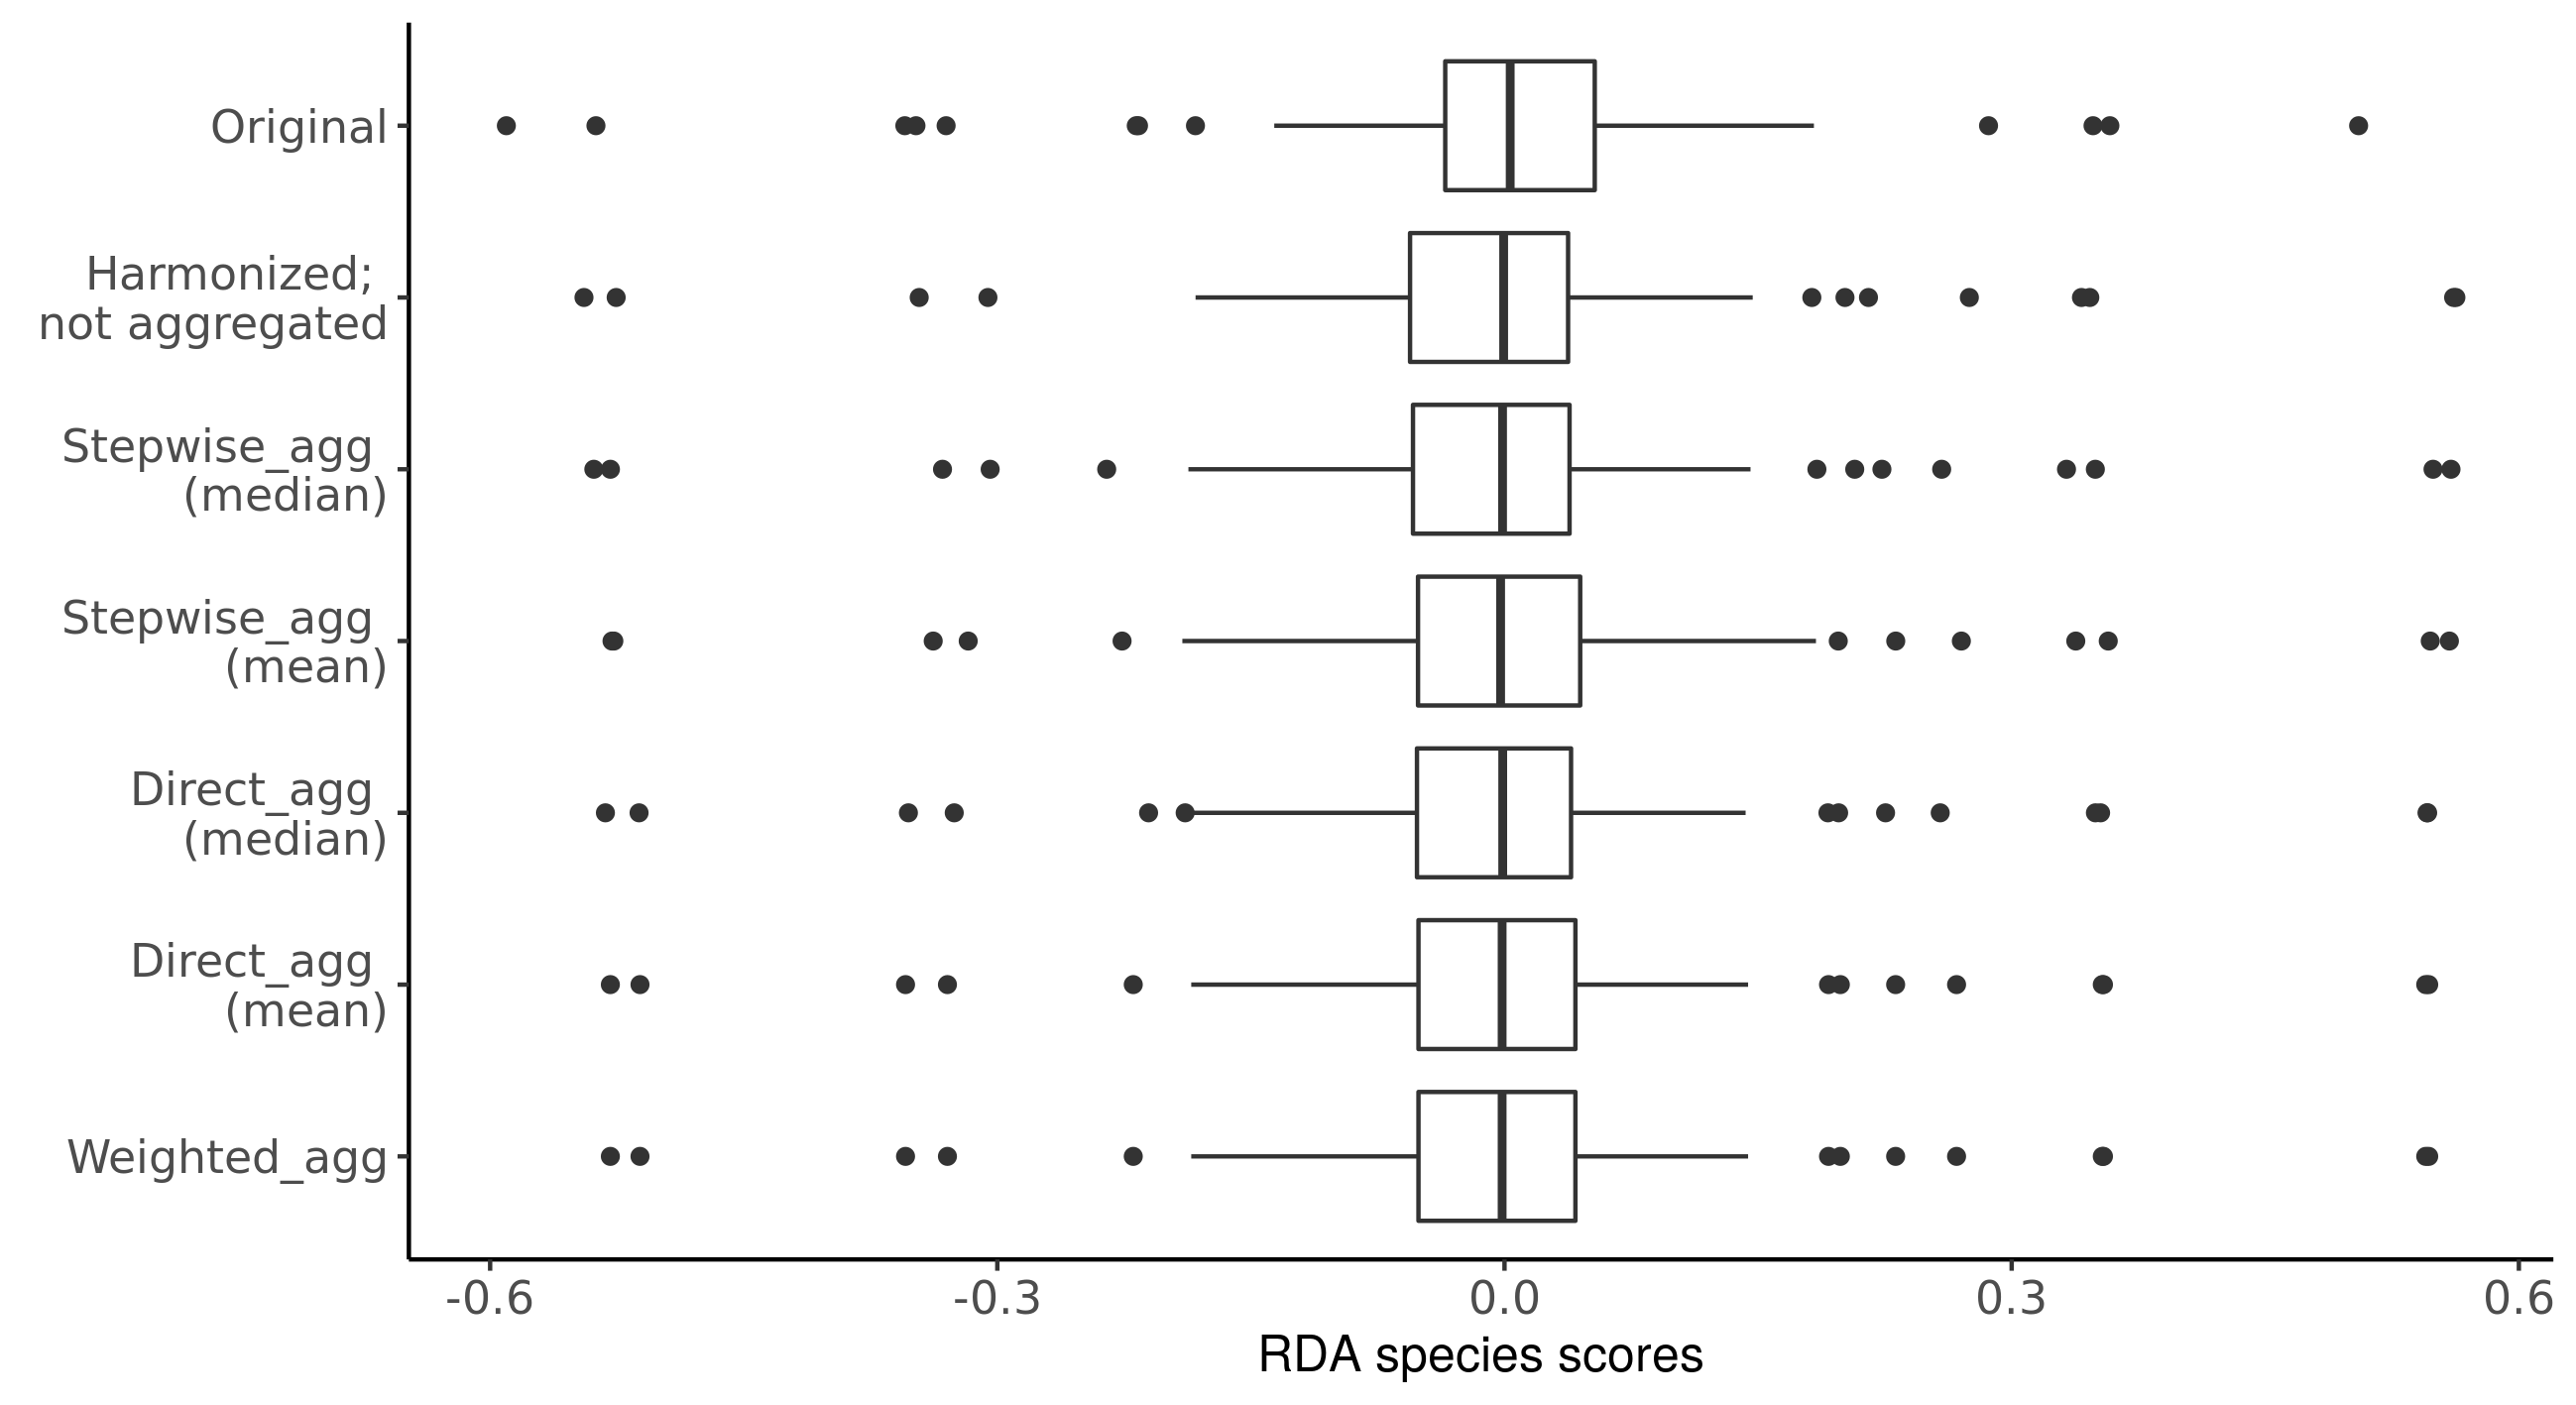
\includegraphics[width=16.5cm, height=10cm]{Species_scores_rda.png}
    \caption{Species scores obtained by RDA from the original analysis (\cite{szocs_effects_2014}), using harmonised grouping features, and using harmonised grouping features with traits aggregated to family level with five different aggregation methods. The dots represent the individual species scores for each analysed trait along the conductivity axis. The violin plot shows the density estimate of the species scores. Grey vertical lines indicate the median of the obtained species scores.}
    \label{fig:violin_plot_species_sc}
\end{figure}

\begin{figure}[H]
  \centering
  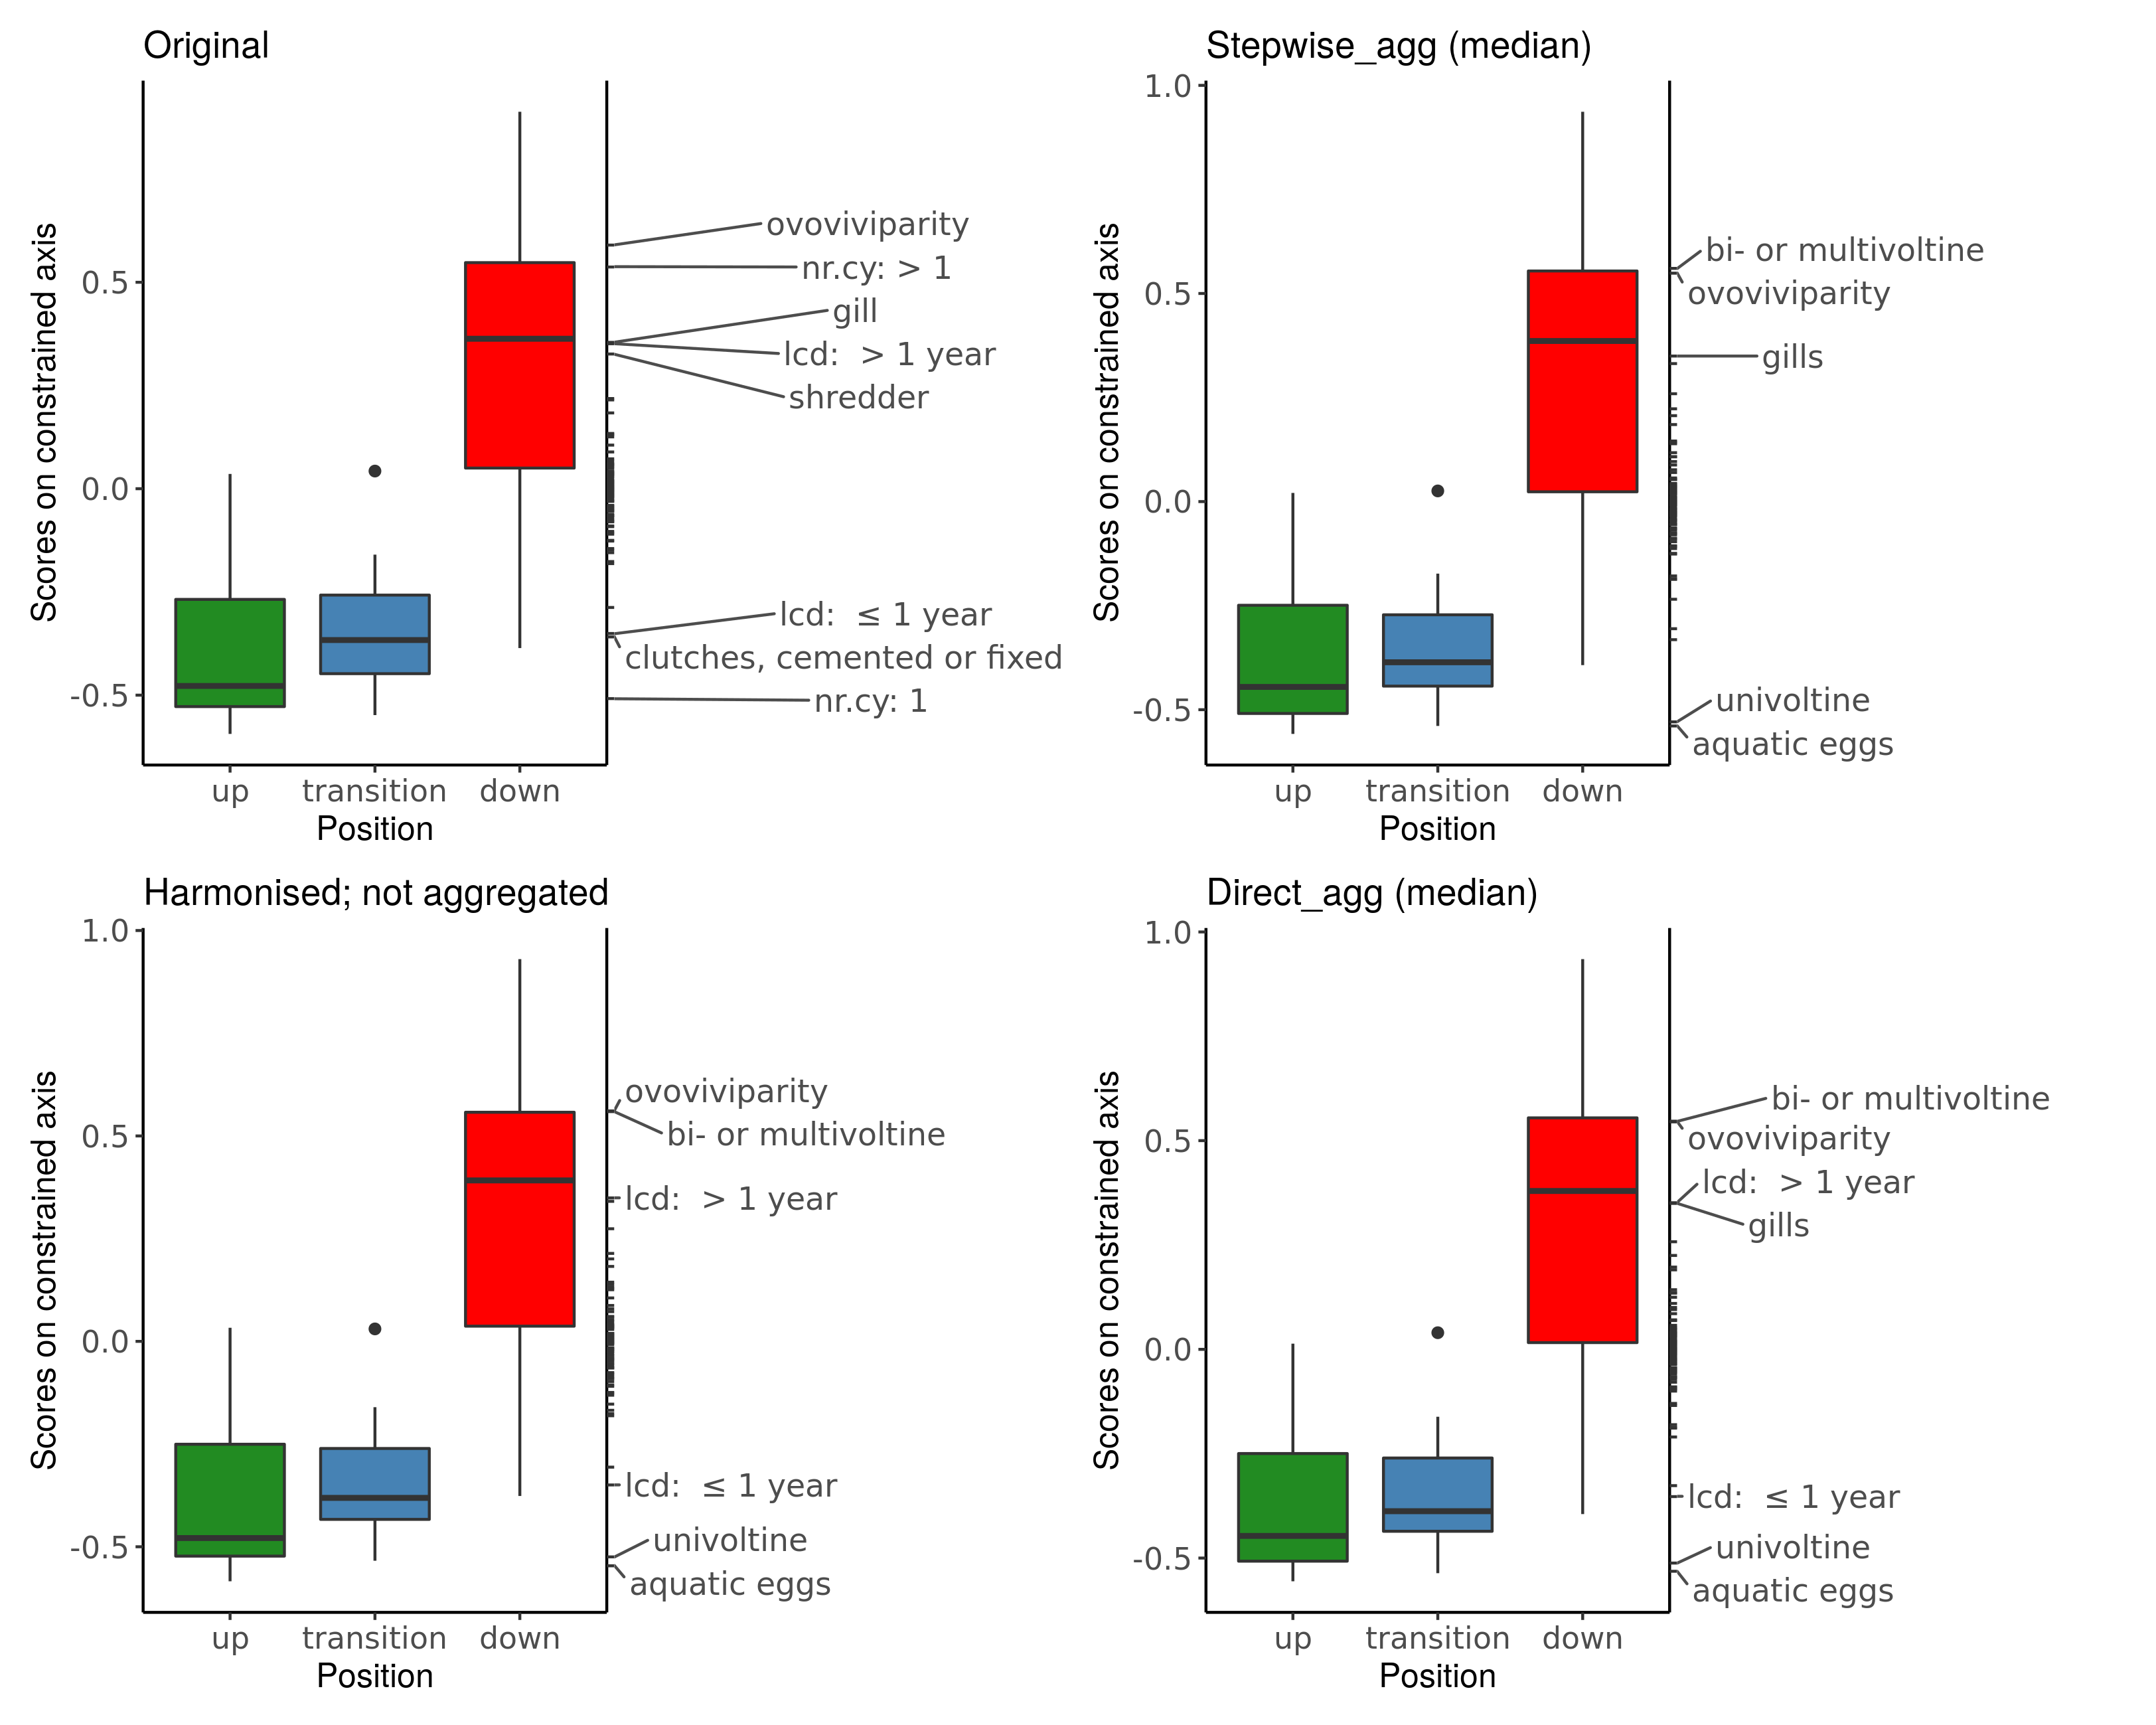
\includegraphics[width=17cm, height=14.5cm]{boxplot_scores_combined.png}
  \caption{RDA of traits constrained by electric conductivity for harmonised but not aggregated data, data aggregated with \textit{stepwise\_agg \textsubscript{median}} (largest difference in terms of responsive traits to salinity to the original study), data aggregated with \textit{direct\_agg \textsubscript{median}} (smallest difference in terms of responsive traits to salinity to the original study), and the original study. Shown are boxplots of the site scores along the conductivity axis. The rug on the right side of each plot indicates species scores of the traits on the conductivity axis. Only traits with a Mahalanobis distance greater than the $97.5 \%$ quantile of the Chi-square distribution (5.02) were labelled. For better comparability, species scores of the original analysis were multiplied by -1. Results for the other aggregated methods are shown in the supporting information (Figure \ref{fig:boxplots_scores_on_constrained_axis_REMAIN}). Abbreviations: lcd, life cycle duration; nr.cy, potential number of cycles per year.}
  \label{fig:boxplot_scores_on_constrained_axis}
\end{figure}

\newpage

%%%%%%%%%%%%%%%%%%%%%%%%%%%%%%%%%%%%%%%%%%%%%%%%%%%%%%%%%%%%%%%%%%%%%%%%%%%%%%%%%%%%%%%%%%%%%%%%%%%%

\section*{Discussion}

% From Freshwater biology: 
% This should highlight the significance of the results and place them in the context of other work. It should not include references to figures or tables cited in the Results – check that all of your Results are presented in the Results section. Figures (e.g. photographs, conceptual diagrams) or tables presented specifically as part of the Discussion are welcome and may be cited there.

Freshwater invertebrate trait databases are a valuable source of data that are freely available to researchers and that can offer opportunities for large-scale, cross-regional ecological study without the need for time-consuming and expensive field work. However, a lack of consistency among regional and continent-wide databases in trait definitions, trait affinity coding, and taxonomic resolution presents challenges to the use of multiple databases for a single study. We explored the effects of harmonising grouping features and aggregating trait affinities at different taxonomic levels from databases from four different continents on the outcomes of trait affinities and on analysis of trait–environment relationships. We found that despite discrepancies in trait definitions and taxonomic resolution across databases, harmonised and aggregated data were useful in identifying trait–environmental relationships, as evidenced by similar results from RDA as were found using observational data. Our results have implications for future multi-regional ecological studies that may benefit from the use of existing databases and provide insight into methods for harmonising traits with differing trait definitions and selecting aggregation methods that minimize either cases or ranges of differences in trait affinity scores when aggregating from higher to lower taxonomic precision.

\subsection*{Harmonising trait databases}

Synthesizing trait information from multiple trait databases is crucial for developing the full potential of trait-based approaches, such as for studying community trait responses to environmental gradients across geographic regions. Others have noted the lack of standardised trait terminology in freshwater ecology (\cite{baird_toward_2011, brink_traits-based_2011}), but we are the first to describe invertebrate trait definition discrepancies for some commonly used grouping features. Our experience can offer some insight into the need for, and process of, harmonising invertebrate trait information from trait databases of different regions. Some of the challenges we found were that grouping features were resolved differently into traits in different databases and that various codings (fuzzy, categorical, binary) were used to describe traits. In addition, the same traits were sometimes defined differently, requiring expert knowledge to reclassify these traits (e.g. the trait piercer). Missing information was another challenge. We aimed to use most of the available invertebrate trait information for different regions to establish harmonised grouping feature datasets, but the availability of trait information varied strongly across grouping features and databases. For instance, there was extensive information available for grouping features that are often used in trait–environment studies, such as feeding mode and respiration, but there was surprisingly little information on body form, a trait that is relatively easy to determine.

To resolve definition discrepancies and facilitate data synthesis in the future, terminological standards are needed. Harmonised definitions and concepts of traits have been developed in the past for other organism groups, such as for plants with the \textit{Thesaurus of Plant Characteristics} (TOP) initiative (\cite{garnier_towards_2017}). The core of this harmonisation initiative is to provide standardised trait definitions and to draw connections to synonyms, related terms, and surrounding concepts by linking to other controlled vocabularies or ontologies in the field. Such initiatives could be a role model for freshwater ecologists to establish unambiguous terminologies for invertebrate traits. The existing freshwater invertebrate trait databases could be linked through standardised terminologies or ontologies, as suggested by \citet{baird_toward_2011}. By following the recently proposed \textit{Ecological Trait-data Standard Vocabulary} (ETS), providers of invertebrate trait data could connect their traits to such ontologies (\cite{schneider_towards_2019}). Once standardised trait definitions are established, these will improve trait data sharing, trait data processing when working with multiple trait databases, and, ultimately, interpretation of the derived results. 

%%%%%%%%%%%%%%%%%%%%%%%%%%%%%%%%%%%%%%%%%%%%%%%%%%%%%%%%%%%%%%%%%%%%%%%%%%%%%%%%%%%%%%%%%%%%%%%%%%%%%%

\subsection*{Trait aggregation method choice}

Observational data for freshwater invertebrates are often resolved to a variety of taxonomic levels because species-level identification can be complicated, time-consuming, and expensive (\cite{marshall_taxonomic_2006, resh_which_2008}). Consequently, trait information at family level has been widely used by freshwater ecologists, for example in bioassessment (\cite{beketov_spear_2009}).
However, assigned traits at family level may not reflect the real trait diversity within, for example, a taxon in the large, ecologically diverse family Chironomidae (\cite{serra_synthesising_2016}). Additionally, various trait aggregation methods have been used by researchers to allow comparison among traits at different taxonomic levels. Evaluation of the differences between aggregated and assigned traits is difficult because it remains unclear what the true value of a particular trait is for a particular family. Aggregation of trait information at species or genus level to a point estimate at family level suggests a precision that is not necessarily present, especially not for traits with high variability or if trait information at species level is missing. Indeed, some traits can vary strongly at more precise taxonomic levels than the family level. For example, \citet{monaghan_improving_2013} found a high intra-family trait dispersion in the Tachet database for traits of the grouping features body size, flow preference, and reproduction. Further, studies focusing on the lability of traits, (i.e. how much traits are constrained by phylogeny), found that traits of ecological preferences (e.g. thermal preference), body size, resistance forms, and, to a lesser extent, feeding mode are labile, and thus possibly highly variable (\cite{poff_functional_2006, wilkes_traitbased_2020}). 

If trait aggregation is necessary, however, our study can offer insight about the circumstances under which the choice of aggregation method may be important. The 5 aggregation methods we tested used either the mean or the median and different weightings to assign family-level affinities. Our results indicated that for both the Australian and North American datasets (1) the median aggregation methods provided affinities that were often closer to the assigned traits than were those provided by the mean aggregation methods and (2) the different weighting approaches exerted only a minor influence on the aggregated trait affinities. However, when differences occurred between median aggregation methods and assigned traits, these differences were greater in absolute value compared with the mean aggregation methods, particularly for the North American dataset where mean absolute differences for median aggregations were twice as high as for mean aggregations. This pattern of greater differences for median than mean aggregations can, in large part, be explained by the binary coding used in the North American trait dataset and by the assigned traits. Binary coded traits have affinities of either 1 or 0; therefore, traits of a particular grouping feature showed, in most cases, a higher difference in trait affinities to each other than if they were fuzzy coded. Median-aggregated binary-coded taxa often resulted in a value of 0 or 1, whereas mean aggregation often yielded values between 0 and 1. Thus, using the median led for the North American dataset either to agreement with the assigned traits or to higher differences compared to the mean aggregation methods. This pattern inherent in using median-aggregation methods to aggregate binary-coded data should be considered when researchers choose methods to resolve affinities at different taxonomic levels. 

We expected that, in addition to averaging measure, different weighting approaches to aggregation (i.e., equal weight to each taxon, equal weight to each genus, or weighted by number of species) would affect affinities for families with varying taxonomic hierarchical structure. However, we found through simulations that although taxonomic structural unevenness appeared to produce variation in affinities among weighting approaches, especially for a family where one genus had a much larger number of species than its other genera, trait variability had a greater effect on the range of affinities (i.e., greater ranges of affinities at higher levels of variance) and on the differences in affinities between weighting methods. Also, the number of differing cases and the mean absolute differences in trait affinities, as well as the distributions of absolute trait affinity differences to assigned traits, were similar across the mean aggregation and across the median aggregation methods, which suggests a small influence of the weighting approach on the aggregation outcomes. The minor impact of the weighting approaches on trait aggregation may be explained by the fact that a considerable portion of taxa had low numbers of genera or species. Of the taxa that were compared from the North American trait dataset, 14 \% were identified at family and 62 \% at genus level, 52 \% comprised five or fewer genera, and 13 \% contained just one genus (Figure \ref{fig:tax_hierarchy_NOA}). In the Australian dataset, 21 \% of the compared taxa were identified at family, 40 \% at genus, and 39 \% at species level, 68 \% of the taxa contained five or fewer genera, and 40 \% just one genus (Figure \ref{fig:tax_hierarchy_AUS}). Hence, these results could change when more species-level trait information becomes available. Our findings show that the choice of aggregation method may matter less when taxonomic hierarchical structure is fairly even and traits are less variable, but the \textit{stepwise\_agg\textsubscript{median}} method tended to produce the widest range in affinities, especially with high taxonomic unevenness and high trait variability. 

\subsection*{Using harmonised and aggregated datasets for ecological research}

By reanalysing trait–environment relationships identified in \citet{szocs_effects_2014} with our harmonised and family-level aggregated datasets, we have illustrated the potential for the use of harmonised and aggregated data in ecological research. As far as we are aware, ours is the first study to compare trait–environment relationships using harmonised and non-harmonised data.
Our re-analysis of the data on salinisation effects on biological traits yielded only slightly different results compared with the original study, which agrees with previous findings that family-level traits can be sensitive enough to detect environmental impacts (\cite{beketov_spear_2009}). However, some of the traits that had responded in the original analysis did not respond in the re-analysis: feeding mode shredder, respiration gills, and life-cycle duration traits. There are several possible reasons for these discrepancies. The non-responsive traits were those closest to the threshold for association with either higher or lower salinity, and so the precision lost through trait harmonisation may have decreased our ability to detect a relatively weak association. Feeding mode shredder was the only trait that was non-responsive when using harmonised (but not aggregated) data as well as when using aggregated data. This result was likely because of the harmonisation procedure, when this trait was combined based on three traits (miner, xylophagus, and shredder). Consequently, the trait affinities in the original data had a higher mean and standard deviation than in the harmonised and aggregated data (Table \ref{tab:SI_resp_traits_summary_stats}), suggesting that the signal in the original data was weakened by harmonisation. Following this result, we suggest that if harmonisation is necessary, harmonised and non-harmonised data, if available, should be compared, and possible averaging effects should be considered in further analyses. However, our results illustrate that where site-level data are not available, harmonised and aggregated datasets may be useful in identifying at least the strongest associations between traits and environmental conditions. 

%%%%%%%%%%%%%%%%%%%%%%%%%%%%%%%%%%%%%%%%%%%%%%%%%%%%%%%%%%%%%%%%%%%%%%%%%%%%%%%%%%%%%%%%%%%%%%%%%%%%%%%

\subsection*{Outlook}

Although comprehensive freshwater invertebrate trait databases have been developed for several regions in the past, data synthesis presents challenges because of discrepancies in trait definitions, coding of trait affinities, and taxonomic resolution. By providing an overview of definition discrepancies, we have set a starting point for the development of standardised trait terminology through which invertebrate trait databases can be linked. Agreement on standard terminology and the subsequent development of ontologies are the next steps to facilitate trait-based analysis at large geographical scales. As our analysis showed, some grouping features might need to be re-classified to fit into such a standardised terminology. Although we showed that trait affinities from fuzzy and binary coding can be used together, we also recommend that a uniform coding of traits should be addressed during trait standardisation. 

As ecological knowledge increases, and with the aid of new  methods such as computer vision for species and trait identification (\cite{hoye_deep_2020}), more observational and species-level trait data may become available in the future, reducing the need for trait aggregation. However, we showed that trait aggregation is often in agreement with expert assignments, especially through aggregation approaches that use the median. No aggregation method is objectively the best, and except for cases where traits are highly variable and taxonomic hierarchical structure is highly uneven, choice of aggregation method does not appear to be influential on the outcome. Weighting trait information based on the taxa present in the database used does not seem to have much influence except when the taxonomic hierarchical structure is highly uneven. However, we recommend that the type of coding used to describe traits (binary, fuzzy) should be considered, because median and mean aggregations can yield very different results for binary-coded traits. We also suggest that a measure of trait dispersion should be reported to indicate the uncertainty of the aggregated estimate. Through the use of carefully synthesised data from freshwater invertebrate trait databases, while acknowledging the limitations inherent in harmonised and aggregated data, the ability to investigate a wide range of large-scale ecological questions is enhanced.
 
%%%%%%%%%%%%%%%%%%%%%%%%%%%%%%%%%%%%%%%%%%%%%%%%%%%%%%%%%%%%%%%%%%%%%%%%%%%%%%%
% Further ideas for the discussion:
% - What do we really know because someone has watched the animals and published their behaviour; what is extrapolated knowledge? 
% - Where does the classification come from? Few sources used in NOA also used in AUS:
% AUS: Merrit \& Cummins 1978/1984 for feeding mode for a few genera and families 
% NOA: Merritt, Richard W., Cummins, Berg 2008 -> but not clear if for feeding mode as well; according to trait description "Cummins, K. W. Trophic Relations of Aquatic Insects" was used for feeding mode
% - Discussion on fuzzy coding -> Uncertainty captured by fuzzy codes? 
% - Extrapolate to "large" scale studies, i.e. studies with a stronger gradient?
% - Traits that responded differently after harmonisation:
% Resp gills: Original data has a lot of zeros, which are not present in the harmonised \& aggregated datasets. In the analysis with the harmonised dataset resp gills is not responding to the salinity gradient. Aggregated data look similar to the harmonised ones, but resp gills is here one of the traits responding to conductivity!
% Why did some aggregated datasets promote life cycle duration traits and others not? Results using trait data obtained when aggregating with stepwise\_agg (median) and stepwise\_agg (mean) indicate that life cycle duration traits are not characterising upstream or downstream sites.
% Results using trait data obtained with the other aggregation methods indicate that life cycle duration traits characterise upstream or downstream sites
% However: Mean, median and SD of these traits are all relatively similar across all aggregated datasets (see Table S2). 
% Include Ben's point? Discussion on evolutionary history?
% Discussion point BK: It is intersting that Australia has fewer species and genus than NOA and EU (not suprisngly since the datasets in Oz were mostly delveoped at family level) but more families than these other regions. I wonder if this indicates that Family richness is really higher in Australia. Perhaps it might be as Australia has a wider range of evolutionary histories. This would be worth considering in the discussion  

%%%%%%%%%%%%%%%%%%%%%%%%%%%%%%%%%%%%%%%%%%%%%%%%%%%%%%%%%%%%%%%%%%%%%%%%%%%%%%%%%%%%%

\section*{Data availability statement}

Harmonised invertebrate trait datasets for Australia, Europe, North America and New Zealand are deposited \textit{Zenondo/Github?}

\section*{Acknowledgments}

% Verena Schreiner body form traits?
We thank Brooke Cassell for technical editing of the manuscript. The project is funded by the German research society (DFG \textit{insert project number}).

\section*{Conflict of interest}

The authors declare no conflict of interest.

\newpage

%%%%%%%%%%%%%%%%%%%%%%%%%%%%%%%%%%%% Bibliography %%%%%%%%%%%%%%%%%%%%%%%%%%%%%%%%%%

\printbibliography

\newpage

%%%%%%%%%%%%%%%%%%%%%%%%%%%%%%%%%%%% Supporting information %%%%%%%%%%%%%%%%%%%%%%%%
\setcounter{table}{0}
\setcounter{figure}{0}
\renewcommand{\thetable}{S\arabic{table}}
\renewcommand{\thefigure}{S\arabic{figure}}

\subfile{Results/SI}



\end{document}